% Options for packages loaded elsewhere
\PassOptionsToPackage{unicode}{hyperref}
\PassOptionsToPackage{hyphens}{url}
\PassOptionsToPackage{dvipsnames,svgnames,x11names}{xcolor}
%
\documentclass[
  11pt,
]{krantz}
\usepackage{amsmath,amssymb}
\usepackage{lmodern}
\usepackage{iftex}
\ifPDFTeX
  \usepackage[T1]{fontenc}
  \usepackage[utf8]{inputenc}
  \usepackage{textcomp} % provide euro and other symbols
\else % if luatex or xetex
  \usepackage{unicode-math}
  \defaultfontfeatures{Scale=MatchLowercase}
  \defaultfontfeatures[\rmfamily]{Ligatures=TeX,Scale=1}
\fi
% Use upquote if available, for straight quotes in verbatim environments
\IfFileExists{upquote.sty}{\usepackage{upquote}}{}
\IfFileExists{microtype.sty}{% use microtype if available
  \usepackage[]{microtype}
  \UseMicrotypeSet[protrusion]{basicmath} % disable protrusion for tt fonts
}{}
\makeatletter
\@ifundefined{KOMAClassName}{% if non-KOMA class
  \IfFileExists{parskip.sty}{%
    \usepackage{parskip}
  }{% else
    \setlength{\parindent}{0pt}
    \setlength{\parskip}{6pt plus 2pt minus 1pt}}
}{% if KOMA class
  \KOMAoptions{parskip=half}}
\makeatother
\usepackage{xcolor}
\IfFileExists{xurl.sty}{\usepackage{xurl}}{} % add URL line breaks if available
\IfFileExists{bookmark.sty}{\usepackage{bookmark}}{\usepackage{hyperref}}
\hypersetup{
  pdftitle={BIcenter: A collaborative Web ETL solution},
  pdfauthor={J. R. Almeida, L. Coelho and J. L. Oliveira},
  colorlinks=true,
  linkcolor={Maroon},
  filecolor={Maroon},
  citecolor={Blue},
  urlcolor={Blue},
  pdfcreator={LaTeX via pandoc}}
\urlstyle{same} % disable monospaced font for URLs
\usepackage{color}
\usepackage{fancyvrb}
\newcommand{\VerbBar}{|}
\newcommand{\VERB}{\Verb[commandchars=\\\{\}]}
\DefineVerbatimEnvironment{Highlighting}{Verbatim}{commandchars=\\\{\}}
% Add ',fontsize=\small' for more characters per line
\usepackage{framed}
\definecolor{shadecolor}{RGB}{248,248,248}
\newenvironment{Shaded}{\begin{snugshade}}{\end{snugshade}}
\newcommand{\AlertTok}[1]{\textcolor[rgb]{0.33,0.33,0.33}{#1}}
\newcommand{\AnnotationTok}[1]{\textcolor[rgb]{0.37,0.37,0.37}{\textbf{\textit{#1}}}}
\newcommand{\AttributeTok}[1]{\textcolor[rgb]{0.61,0.61,0.61}{#1}}
\newcommand{\BaseNTok}[1]{\textcolor[rgb]{0.06,0.06,0.06}{#1}}
\newcommand{\BuiltInTok}[1]{#1}
\newcommand{\CharTok}[1]{\textcolor[rgb]{0.5,0.5,0.5}{#1}}
\newcommand{\CommentTok}[1]{\textcolor[rgb]{0.37,0.37,0.37}{\textit{#1}}}
\newcommand{\CommentVarTok}[1]{\textcolor[rgb]{0.37,0.37,0.37}{\textbf{\textit{#1}}}}
\newcommand{\ConstantTok}[1]{\textcolor[rgb]{0,0,0}{#1}}
\newcommand{\ControlFlowTok}[1]{\textcolor[rgb]{0.27,0.27,0.27}{\textbf{#1}}}
\newcommand{\DataTypeTok}[1]{\textcolor[rgb]{0.27,0.27,0.27}{#1}}
\newcommand{\DecValTok}[1]{\textcolor[rgb]{0.06,0.06,0.06}{#1}}
\newcommand{\DocumentationTok}[1]{\textcolor[rgb]{0.37,0.37,0.37}{\textbf{\textit{#1}}}}
\newcommand{\ErrorTok}[1]{\textcolor[rgb]{0.14,0.14,0.14}{\textbf{#1}}}
\newcommand{\ExtensionTok}[1]{#1}
\newcommand{\FloatTok}[1]{\textcolor[rgb]{0.06,0.06,0.06}{#1}}
\newcommand{\FunctionTok}[1]{\textcolor[rgb]{0,0,0}{#1}}
\newcommand{\ImportTok}[1]{#1}
\newcommand{\InformationTok}[1]{\textcolor[rgb]{0.37,0.37,0.37}{\textbf{\textit{#1}}}}
\newcommand{\KeywordTok}[1]{\textcolor[rgb]{0.27,0.27,0.27}{\textbf{#1}}}
\newcommand{\NormalTok}[1]{#1}
\newcommand{\OperatorTok}[1]{\textcolor[rgb]{0.43,0.43,0.43}{\textbf{#1}}}
\newcommand{\OtherTok}[1]{\textcolor[rgb]{0.37,0.37,0.37}{#1}}
\newcommand{\PreprocessorTok}[1]{\textcolor[rgb]{0.37,0.37,0.37}{\textit{#1}}}
\newcommand{\RegionMarkerTok}[1]{#1}
\newcommand{\SpecialCharTok}[1]{\textcolor[rgb]{0,0,0}{#1}}
\newcommand{\SpecialStringTok}[1]{\textcolor[rgb]{0.5,0.5,0.5}{#1}}
\newcommand{\StringTok}[1]{\textcolor[rgb]{0.5,0.5,0.5}{#1}}
\newcommand{\VariableTok}[1]{\textcolor[rgb]{0,0,0}{#1}}
\newcommand{\VerbatimStringTok}[1]{\textcolor[rgb]{0.5,0.5,0.5}{#1}}
\newcommand{\WarningTok}[1]{\textcolor[rgb]{0.37,0.37,0.37}{\textbf{\textit{#1}}}}
\usepackage{longtable,booktabs,array}
\usepackage{calc} % for calculating minipage widths
% Correct order of tables after \paragraph or \subparagraph
\usepackage{etoolbox}
\makeatletter
\patchcmd\longtable{\par}{\if@noskipsec\mbox{}\fi\par}{}{}
\makeatother
% Allow footnotes in longtable head/foot
\IfFileExists{footnotehyper.sty}{\usepackage{footnotehyper}}{\usepackage{footnote}}
\makesavenoteenv{longtable}
\usepackage{graphicx}
\makeatletter
\def\maxwidth{\ifdim\Gin@nat@width>\linewidth\linewidth\else\Gin@nat@width\fi}
\def\maxheight{\ifdim\Gin@nat@height>\textheight\textheight\else\Gin@nat@height\fi}
\makeatother
% Scale images if necessary, so that they will not overflow the page
% margins by default, and it is still possible to overwrite the defaults
% using explicit options in \includegraphics[width, height, ...]{}
\setkeys{Gin}{width=\maxwidth,height=\maxheight,keepaspectratio}
% Set default figure placement to htbp
\makeatletter
\def\fps@figure{htbp}
\makeatother
\setlength{\emergencystretch}{3em} % prevent overfull lines
\providecommand{\tightlist}{%
  \setlength{\itemsep}{0pt}\setlength{\parskip}{0pt}}
\setcounter{secnumdepth}{5}
\usepackage{booktabs}
\usepackage{longtable}
\usepackage[bf,singlelinecheck=off]{caption}

\usepackage{framed,color}
\definecolor{shadecolor}{RGB}{248,248,248}

\renewcommand{\textfraction}{0.05}
\renewcommand{\topfraction}{0.8}
\renewcommand{\bottomfraction}{0.8}
\renewcommand{\floatpagefraction}{0.75}

\renewenvironment{quote}{\begin{VF}}{\end{VF}}
\let\oldhref\href
\renewcommand{\href}[2]{#2\footnote{\url{#1}}}

\ifxetex
  \usepackage{letltxmacro}
  \setlength{\XeTeXLinkMargin}{1pt}
  \LetLtxMacro\SavedIncludeGraphics\includegraphics
  \def\includegraphics#1#{% #1 catches optional stuff (star/opt. arg.)
    \IncludeGraphicsAux{#1}%
  }%
  \newcommand*{\IncludeGraphicsAux}[2]{%
    \XeTeXLinkBox{%
      \SavedIncludeGraphics#1{#2}%
    }%
  }%
\fi

\usepackage{makeidx}
\makeindex

\urlstyle{tt}

\usepackage{amsthm}
\makeatletter
\def\thm@space@setup{%
  \thm@preskip=8pt plus 2pt minus 4pt
  \thm@postskip=\thm@preskip
}
\makeatother

\frontmatter
\ifLuaTeX
  \usepackage{selnolig}  % disable illegal ligatures
\fi
\usepackage[]{natbib}
\bibliographystyle{apalike}

\title{BIcenter: A collaborative Web ETL solution}
\author{J. R. Almeida, L. Coelho and J. L. Oliveira}
\date{2021-10-18}

\begin{document}
\maketitle

{
\hypersetup{linkcolor=}
\setcounter{tocdepth}{1}
\tableofcontents
}
\listoffigures
\listoftables
\hypertarget{preface}{%
\chapter*{Preface}\label{preface}}


\mainmatter

\hypertarget{introduction}{%
\chapter{Introduction}\label{introduction}}

BIcenter is a web-based platform that allows the building and management of ETL pipelines, by non-IT users, in a multi-institution environment. Each institution manages and mantains ETL tasks and provides the resources for the execution of the associated tasks. Thus, each institution owns its private data sources, servers for ETL task execution and a task scheduler that allows periodic execution. In order to provide access and management control of ETL tasks and institutions, there are four distinct types of users:

\begin{itemize}
\tightlist
\item
  Administrator: Entity that moderates the platform. This actor has permissions to create and delete institutions.
\item
  Resource Manager: Entity that manages private data sources and execution servers. This actor has permissions to create and delete private data sources and execution servers, within specific institutions.
\item
  Task Manager: Entity that builds and executes ETL tasks. This actor can create and configure ETL tasks, within specific institutions.
\item
  Data Analyst: This actor has permissions to inspect task execution history, namely the resulting data, execution logs and performance metrics.
\end{itemize}

\hypertarget{main-requirements}{%
\section{Main requirements}\label{main-requirements}}

\textbf{Information Security}
Since ETL tasks parse and handle sensitive data that belongs to a particular institution, the system must be designed and implemented taking in account these security issues, namely user authentication, access control, data protection and isolation.

\textbf{System Reliability}
Considering the periodic execution of ETL tasks, it is important to ensure that each execution is correctly initialized, started, motorized and concluded. When some fatal error occurs during an ETL task execution, the system must be able to handle the error and successfully conclude the execution.

\textbf{Solution Scalability}
Since a complete ETL tool typically encompasses a wide variety of components, it is crucial to build an agile approach to the development and integration of new ETL components.

\hypertarget{system-implementation}{%
\chapter{System Implementation}\label{system-implementation}}

This chapter contains the description of the main aspects of BIcenter implementation.

\hypertarget{requirements}{%
\section{Requirements}\label{requirements}}

The main goal of this application was to allow the building and management of ETL pipelines, by non-IT users, in a multi-institution environment. Therefore, some functional requirements were were considered to implement a proper and reliable solution.

Each institution manages and mantains ETL tasks and provides the resources for the execution of the associated tasks. Thus, each institution owns its private data sources, servers for ETL task execution and a task scheduler that allows periodic execution. In order to provide access and management control of ETL tasks and institutions, there are four distinct types of users: 1) Administrator, entity that moderates the platform, and it has permissions to create and delete institutions; 2) Resource Manager, entity that manages private data sources and execution servers, and it has permissions to create and delete private data sources and execution servers, within specific institutions; 3) Task Manager, entity that builds and executes ETL tasks, and it can create and configure ETL tasks, within specific institutions; and 4) Data Analyst, actor with permissions to inspect task execution history, namely the resulting data, execution logs and performance metrics.

The functional model was derived from the identification of all key components from a top-down analysis of the system requirements. Figure \ref{fig:workflow} illustrates step by step all actions and interactions between the main actors in order to build and execute ETL tasks and to analyze the output results. Firstly, the administrator must create an institution. A resource manager with access to the institution can create and configure all desired private data sources and task execution servers. Thereafter, a task manager can build and configure the ETL task and then schedule it for periodic or non-periodic execution. At the configured times the task will be sent to the execution server and executed. At the end of the execution, a notification will be sent to the data analysts, so they can check the execution results.

\begin{figure}
\centering
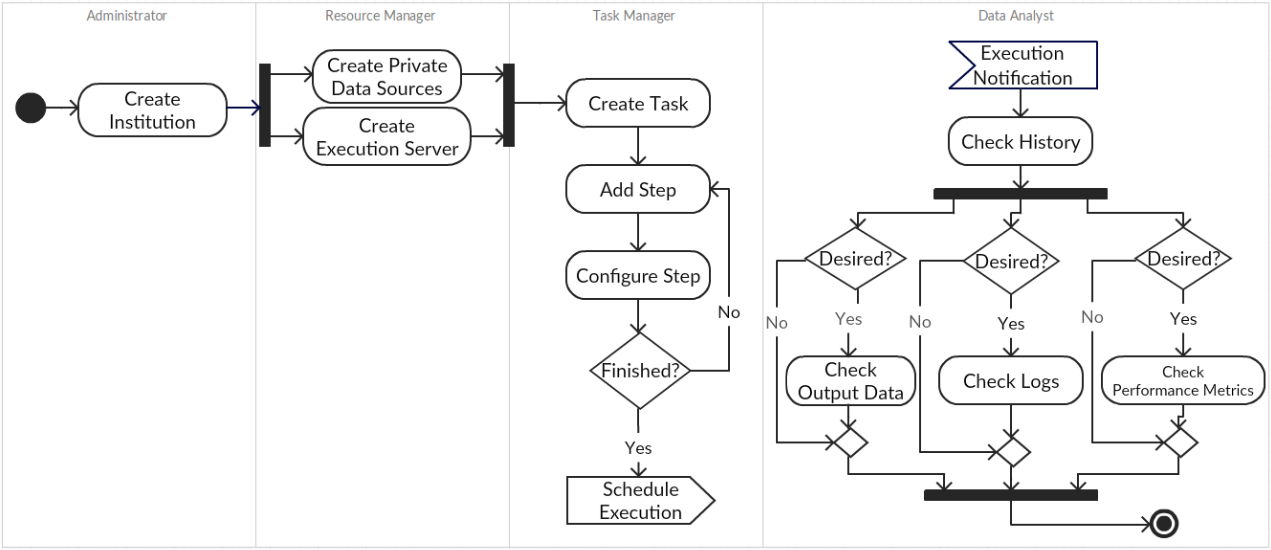
\includegraphics{images/workflow.png}
\caption{\label{fig:workflow} System workfow to build, manage and execute ETL tasks.}
\end{figure}

\hypertarget{architecture}{%
\section{Architecture}\label{architecture}}

The architecture considers four different tiers: 1) Application tier controls all application functionalities and maintains the system business logic; 2) Data tier is responsible for the maintenance of the private data sources; 3) Processing tier has the duty of executing and monitoring ETL task executions; and 4) Client tier is responsible for the solution presentation and page rendering. Figure \ref{fig:architecture} illustrates this architecture.

\begin{figure}
\centering
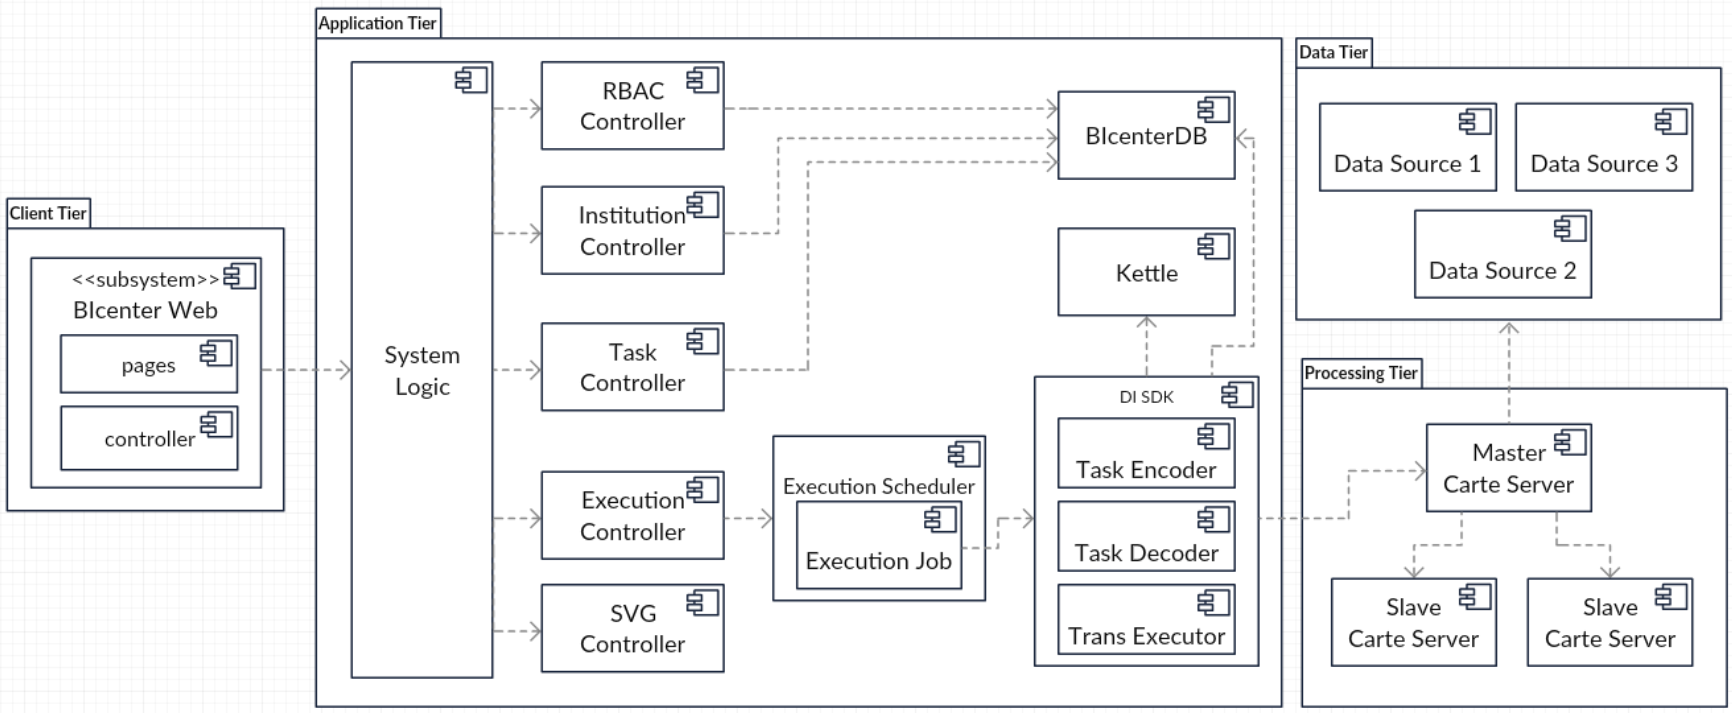
\includegraphics{images/architecture.png}
\caption{\label{fig:architecture} Components diagram of system architecture.}
\end{figure}

The system logic is built upon five different controllers: 1) RBAC controller provides user identity and evaluates access requests to resources; 2) Institution controller allows the creation and destruction of institutions, and resource allocation in institutions; 4) Task controller enables the creation, configuration and destruction of ETL tasks; and 5) Execution controller uses Kettle and Carte servers, so it can build, remotely execute and monitor ETL tasks.

Data Integration (DI) Software Development Kit (SDK) seeks to bridge the gap between Kettle and the stored information in BIcenter database (DB). It provides methods to build Pentaho's ETL processes according to the stored information, and also to execute them. Nevertheless, task execution is a periodic process. Therefore, Execution Scheduler manages the task execution scheduling. When the appropriated time arrives, a Execution Job is triggered. That job will communicate with DI SDK so that the given task is indeed executed. SVG controller maps between images and components, with the intent to build the visual pipeline.

BIcenter Web client adopted Model-View-Controller (MVC) architectural pattern. This pattern divides the web application in three different components:

\begin{itemize}
\tightlist
\item
  Model: represents the knowledge and data in an application. It has the responsability to respond to information requests, proceed to information changes according to given instructions requests, and to notify observers in event-driven systems when information changes. Typically, the application data is stored in a database.
\item
  View: it represents the user interface. The View updates the UI upon changes in the Model, by rendering the data into the suitable UI form.
\item
  Controller: it handles events that occurs in the View, such as user interactions, and updates the Model accordingly.
\end{itemize}

\hypertarget{etl-sdk}{%
\section{ETL SDK}\label{etl-sdk}}

The ETL Task Editor was idealized to allow users to build a visual representation of the desired ETL pipeline. This editor must be able to process a similar structure to the ones used by the desktop ETL tools and generate the correspondent visual representation of the ETL task. MxGraph was used to build the ETL pipeline editor, and this Java/JavaScript diagramming library enables the building of interactive graphs. A graph consists in a set of cells. A cell can either be a vertex or an hop. Thus, a graph is formed by a group of vertices connected by edges. The vertices correspond to the ETL steps and the edges correspond to the ETL hops. Hence, in order to exhibit the desired task within the mxEditor, it is necessary to translate the task to the corresponding mxGraph object. GraphDecoder is responsible for creating a mxGraph and defining the appropriated model, according to the given Task. To insert vertices and edges in the graph model, a transaction must be created (beginUpdate and endUpdate). This is required for the model to remain in a consistent state. A default parent is automatically created and represents the first child of the root cell in the model. Subsequent elements must be added to the default parent.

The ETL SDK was built on top of PDI SDK. Kettle contains a rich set of data integration functionality that is exposed in a set of data integration tools. However, we can also use Kettle as a library in our own software and solutions. Pentaho Data Integration can be used as a Java API composed by three main components: 1) Core, that contains the core classes for Kettle; 2) Database, that contains the database-related classes; and 3) Engine, that contains the Kettle's runtime classes.

Figure \ref{fig:kettle} explains step by step how an ETL task is executed. The initialization of the Kettle environment loads all available plugins, initializes the logging environment and set up and reads the system variables. After the environment initialization, the transformation metadata is loaded and a transformation engine object is instantiated. Then, the execution is prepared and the transformation threads are started. Finally, because the whole transformation runs multi- threaded, it waits until all processing is completed.

\begin{figure}
\centering
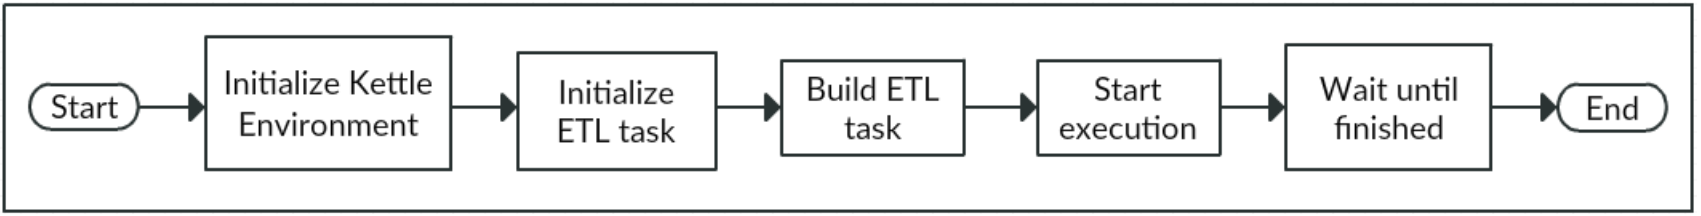
\includegraphics{images/kettle.png}
\caption{\label{fig:kettle} ETL task execution flowchart.}
\end{figure}

In Kettle, an ETL process can be represented by six classes {[}31{]}:

\begin{itemize}
\tightlist
\item
  TransMeta: is the class that defines the information about the ETL process and offers methods to save and load it from XML, as well as methods to alter an ETL process by adding/removing databases, steps, hops, etc.
\item
  Trans: represents the information and operations associated with the concept of an ETL process. It can loads, instantiates, initializes, runs, and monitors the execution of the ETL process.
\item
  DatabaseMeta: defines the database specific parameters for a certain database type.
\item
  StepMeta: is the class that defines the information about a ETL process's Step.
\item
  TransHopMeta: defines a link between two steps in an ETL process.
\item
  BaseStep: represents the information and operations associated with the concept of an ETL process Step. It offers initialization, row processing and step clean-up methods.
\end{itemize}

Initially a TransMeta must be properly configured with all proper DatabaseMetas, StepMetas and TransHopMetas. TransDecoder is responsible to create a TransMeta and define all underlying information, according to the given Task. GenericStep is a class that has a generic algorithm to encode or decode a given Step to or from a Kettle's StepMeta. In order to provide interface segregation, TransDecoder must use the StepDecoder interface that only provides the GenericStep decoding method.

After having a correctly configured TransMeta, it can be executed with the associated Trans object. TransExecutor is a singleton responsible for the initialization, execution and monitoring of the Trans object. Moreover, it writes and stores the execution logs, step measures and status, and the resulting data in real-time. To accomplish this, listeners are coupled to the Trans and Steps objects in order to obtain the results and metrics throughout the transformation's execution.

\hypertarget{software-user-manual}{%
\chapter{Software User Manual}\label{software-user-manual}}

This chapter presents the main interfaces of BIcenter, aiming to help users to navigate through the system.

\hypertarget{initial-views}{%
\section{Initial views}\label{initial-views}}

The login page presented in Figure \ref{fig:login} allows users to be authenticated using their credentials. This can be connected with the institution LDAP, which provides a central place to store usernames and passwords.

\begin{figure}
\centering
\includegraphics{images/login.png}
\caption{\label{fig:login} Login page.}
\end{figure}

After the authentication process, the user is redirected to the application's home page represented in Figure \ref{fig:home}. This page contains all the institutions that the user belongs to. In this case, this user has permission to create a new instance of an institution in the application using the modal illustrated in Figure \ref{fig:newinstitution}.

\begin{figure}
\centering
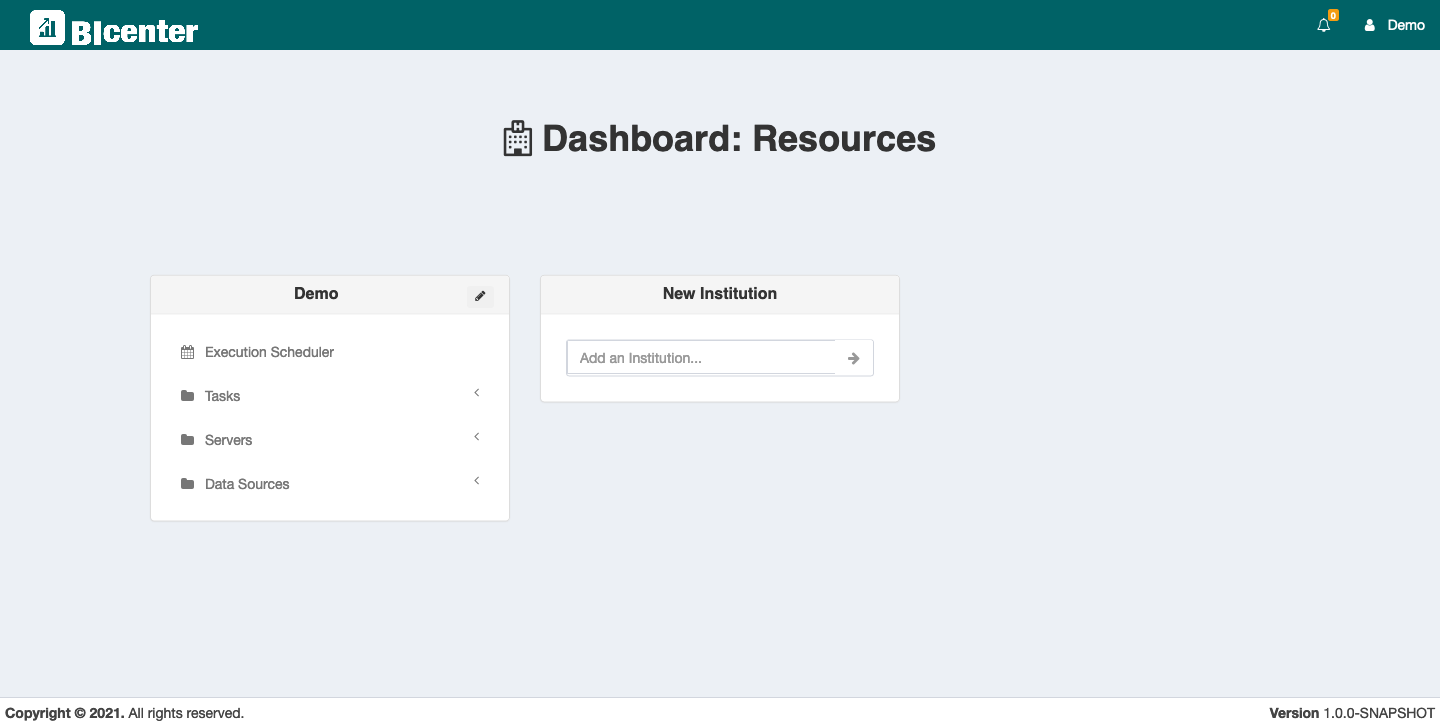
\includegraphics{images/home.png}
\caption{\label{fig:home} Home page after login with all institutions assigned to the user.}
\end{figure}

\begin{figure}
\centering
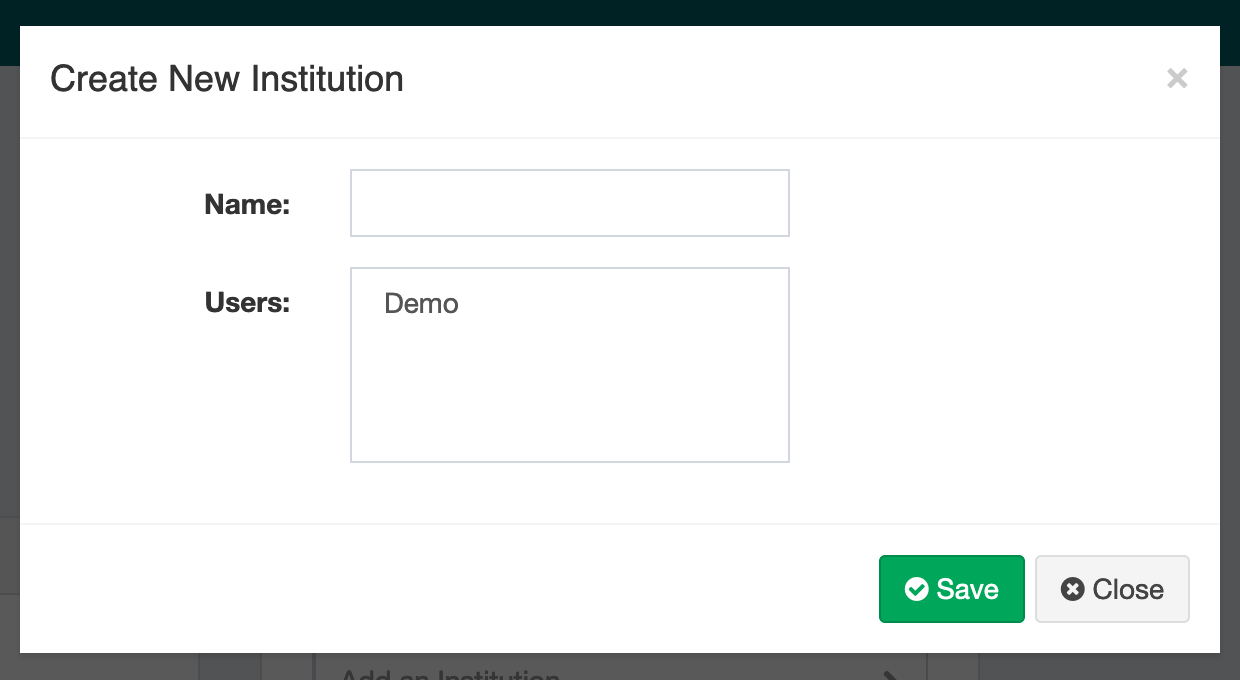
\includegraphics[width=0.75\textwidth,height=\textheight]{images/newInstitution.png}
\caption{\label{fig:newinstitution} Modal to create new institution.}
\end{figure}

\hypertarget{institutional-features}{%
\section{Institutional features}\label{institutional-features}}

The configuration of a data source is illustrated in Figures \ref{fig:newds1} and \ref{fig:newds2}. Firstly is created the data source instance in the institution, and then, the details of this connection are inserted in the modal represented in Figure \ref{fig:newds2}.

\begin{figure}
\centering
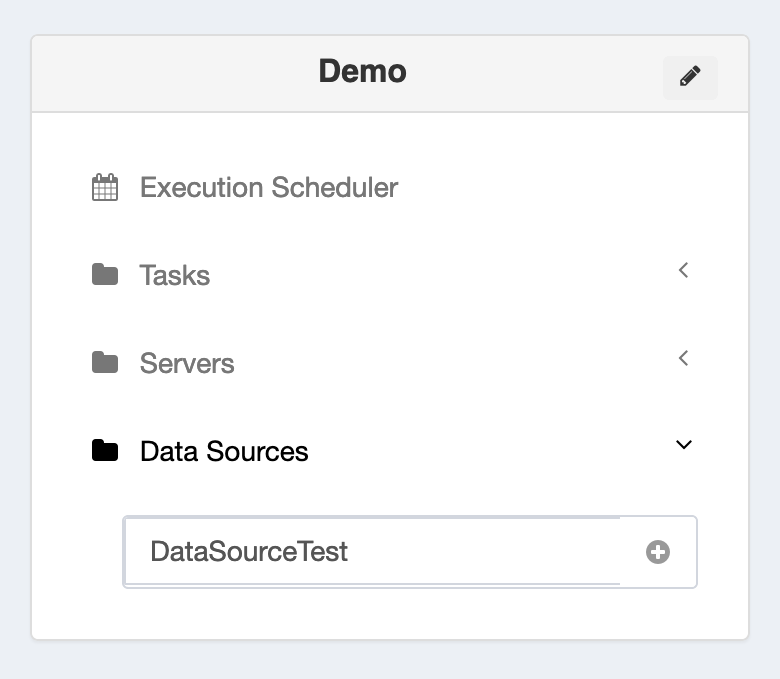
\includegraphics[width=0.5\textwidth,height=\textheight]{images/newDataSource1.png}
\caption{\label{fig:newds1} Creation of connection to a data source (first step).}
\end{figure}

\begin{figure}
\centering
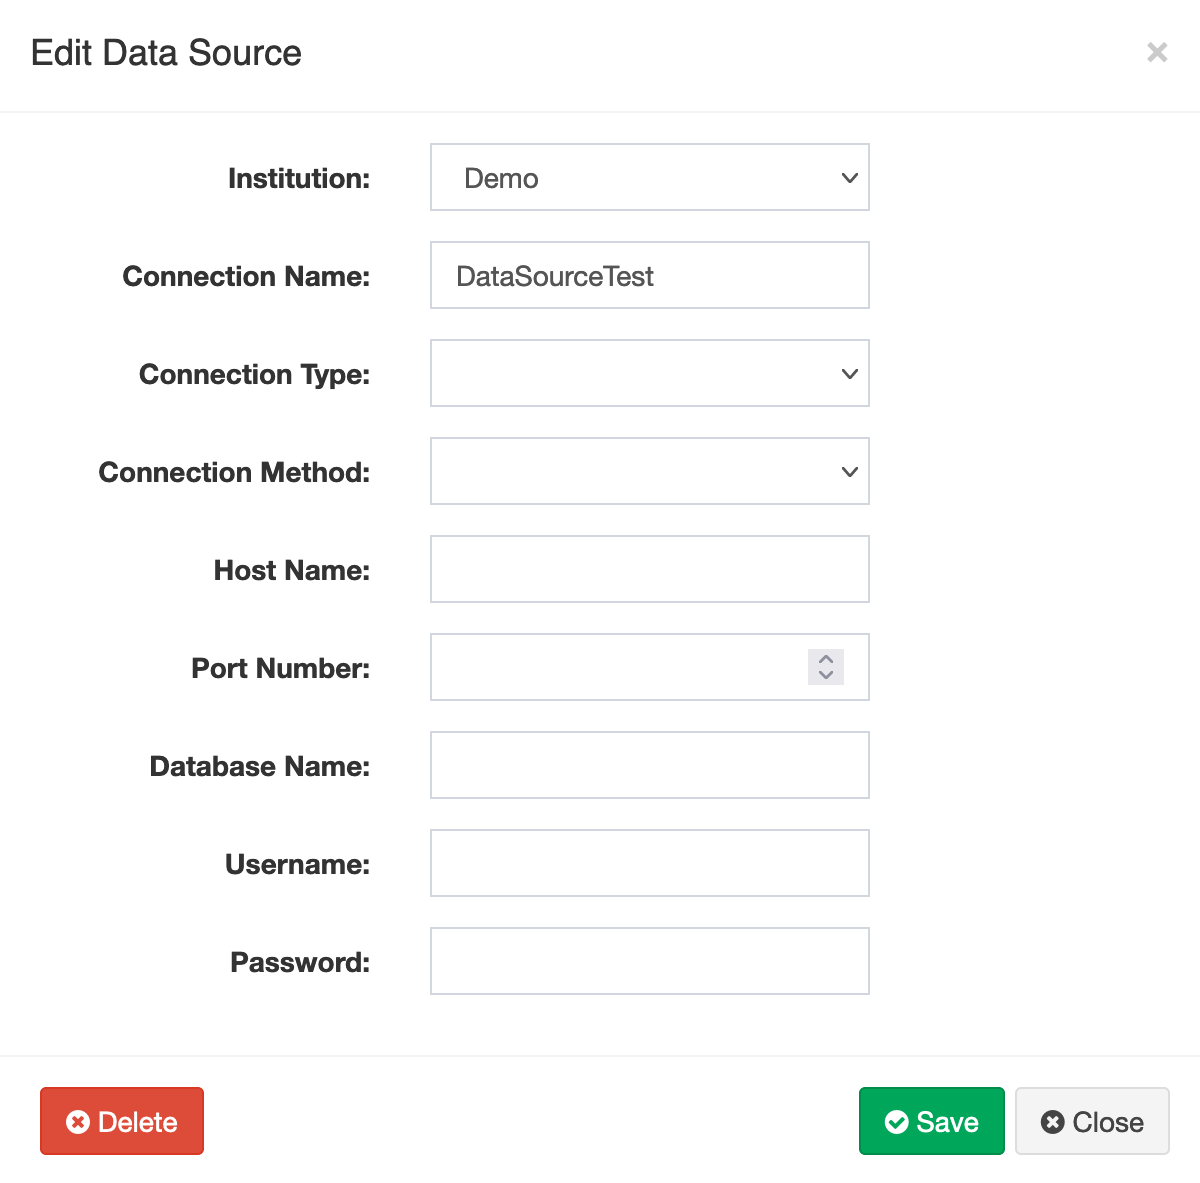
\includegraphics[width=0.75\textwidth,height=\textheight]{images/newDataSource2.png}
\caption{\label{fig:newds2} Modal to insert information regarding the new connection to a data source (second step).}
\end{figure}

The connection to the remote server follows a similar flow. This configuration is illustrated in Figures \ref{fig:newserver1} and \ref{fig:newserver2}.

\begin{figure}
\centering
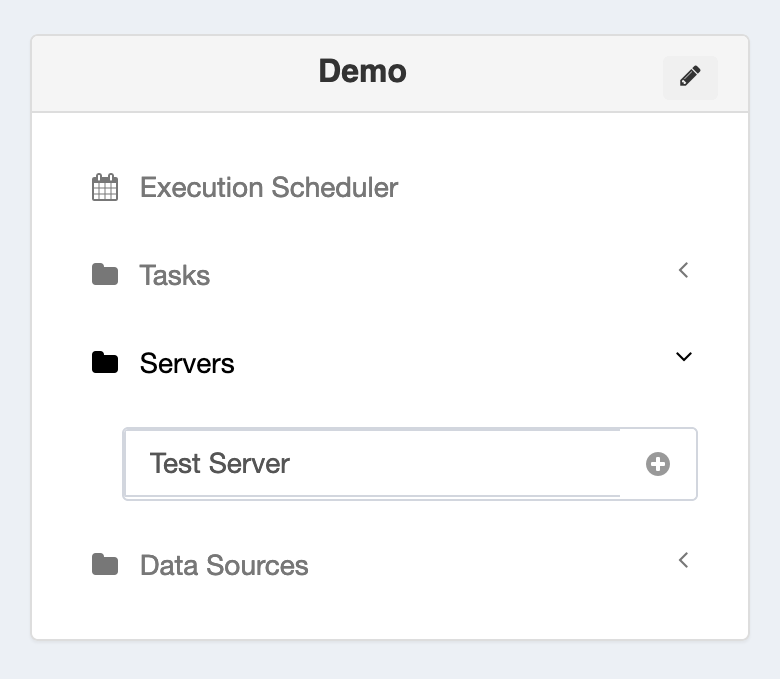
\includegraphics[width=0.5\textwidth,height=\textheight]{images/newServer1.png}
\caption{\label{fig:newserver1} Creation of connection to a remote server (first step).}
\end{figure}

\begin{figure}
\centering
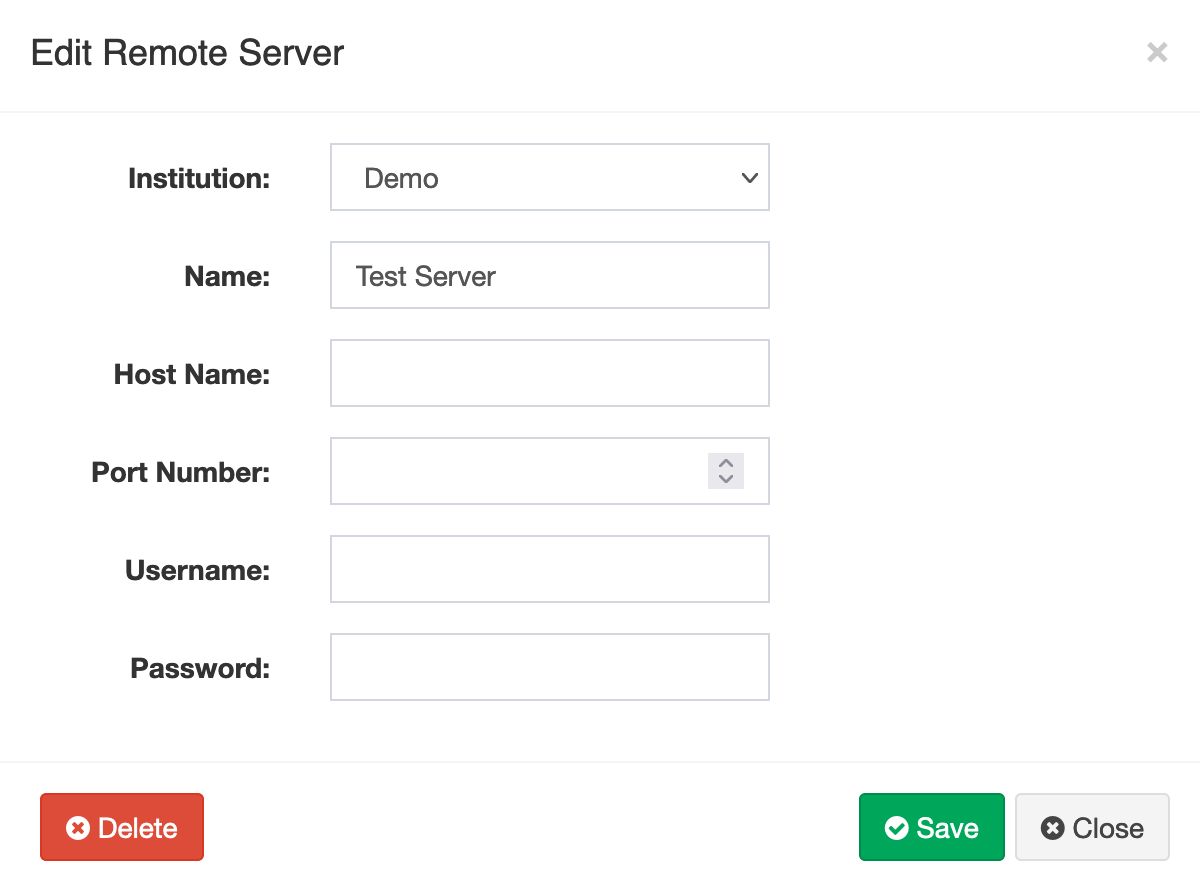
\includegraphics[width=0.75\textwidth,height=\textheight]{images/newServer2.png}
\caption{\label{fig:newserver2} Modal to insert information regarding the new connection to a remote server (second step).}
\end{figure}

Finally, the ETL tasks are also created for the institutions. This feature redirects the users to the ETL Task Editor, in which they can design and implement an ETL pipeline using the web interface. The creation of a new task can be done by using the option represented in Figure \ref{fig:newtask}.

\begin{figure}
\centering
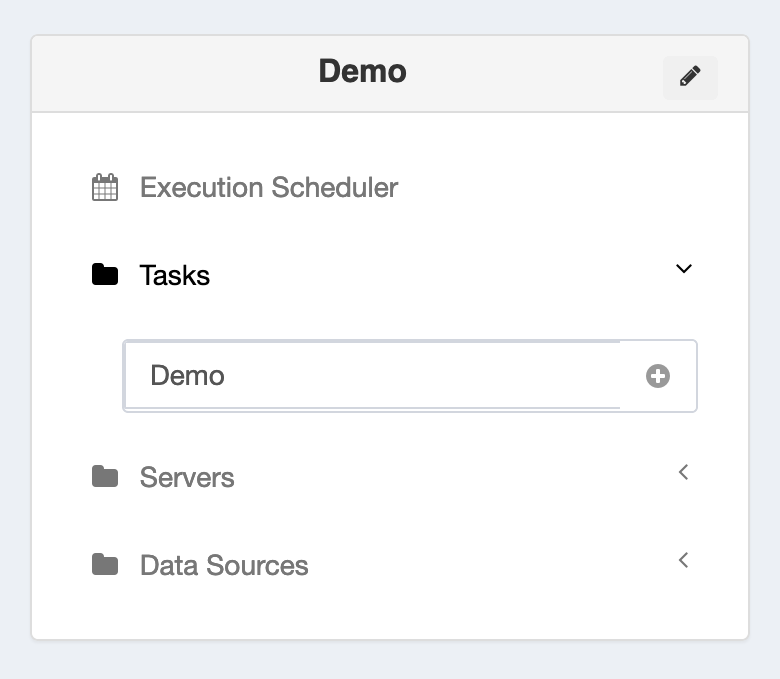
\includegraphics[width=0.5\textwidth,height=\textheight]{images/newTask.png}
\caption{\label{fig:newtask} Creation of a new ETL task (first step).}
\end{figure}

\hypertarget{etl-task-editor}{%
\section{ETL Task Editor}\label{etl-task-editor}}

The ETL Task Editor allows users to create an ETL pipeline by dragging and dropping ETL components. Figure \ref{fig:editor} shows an overview of this web editor.

\begin{figure}
\centering
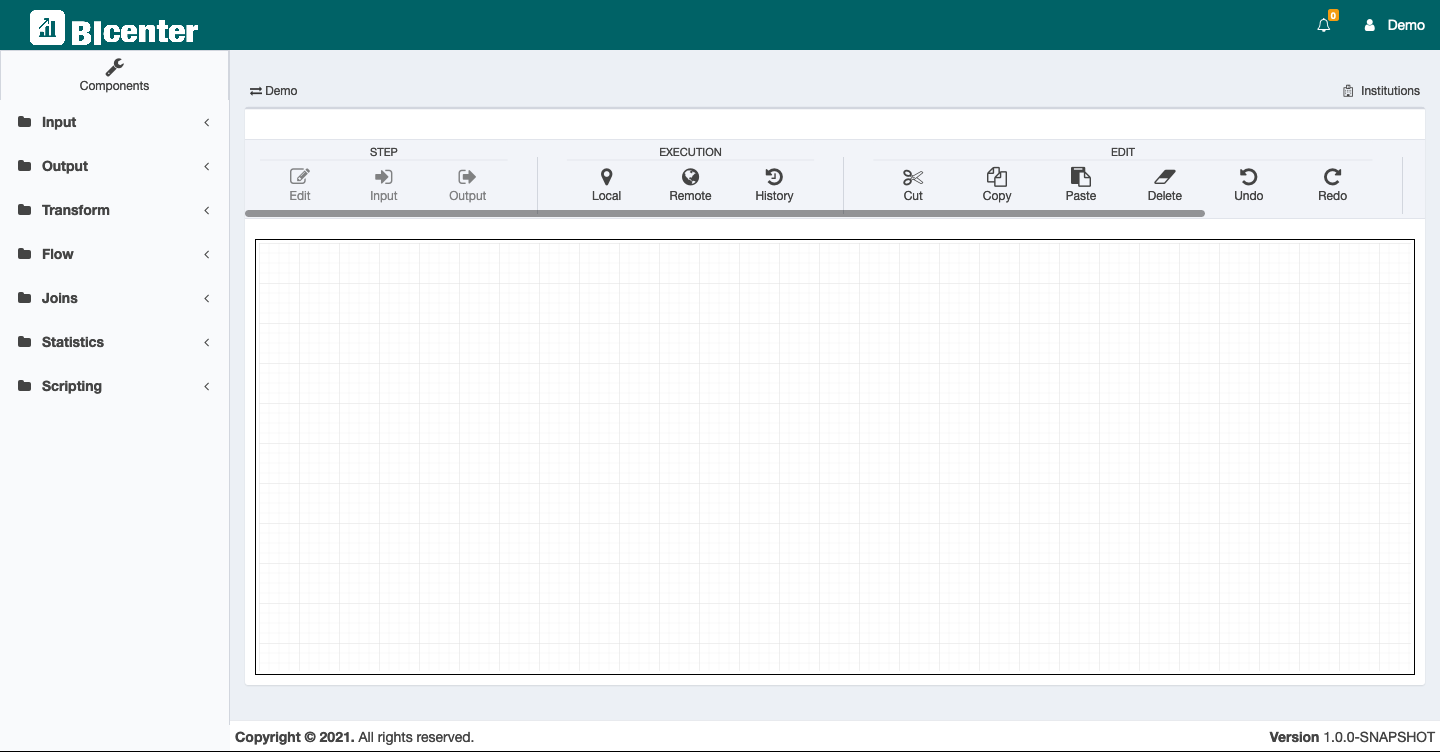
\includegraphics{images/editor.png}
\caption{\label{fig:editor} Overview of the ETL Task Editor.}
\end{figure}

Figure \label{fig:example} shows an example of an ETL pipeline implemented in the ETL Task Editor using the four most common ETL components.

\begin{figure}
\centering
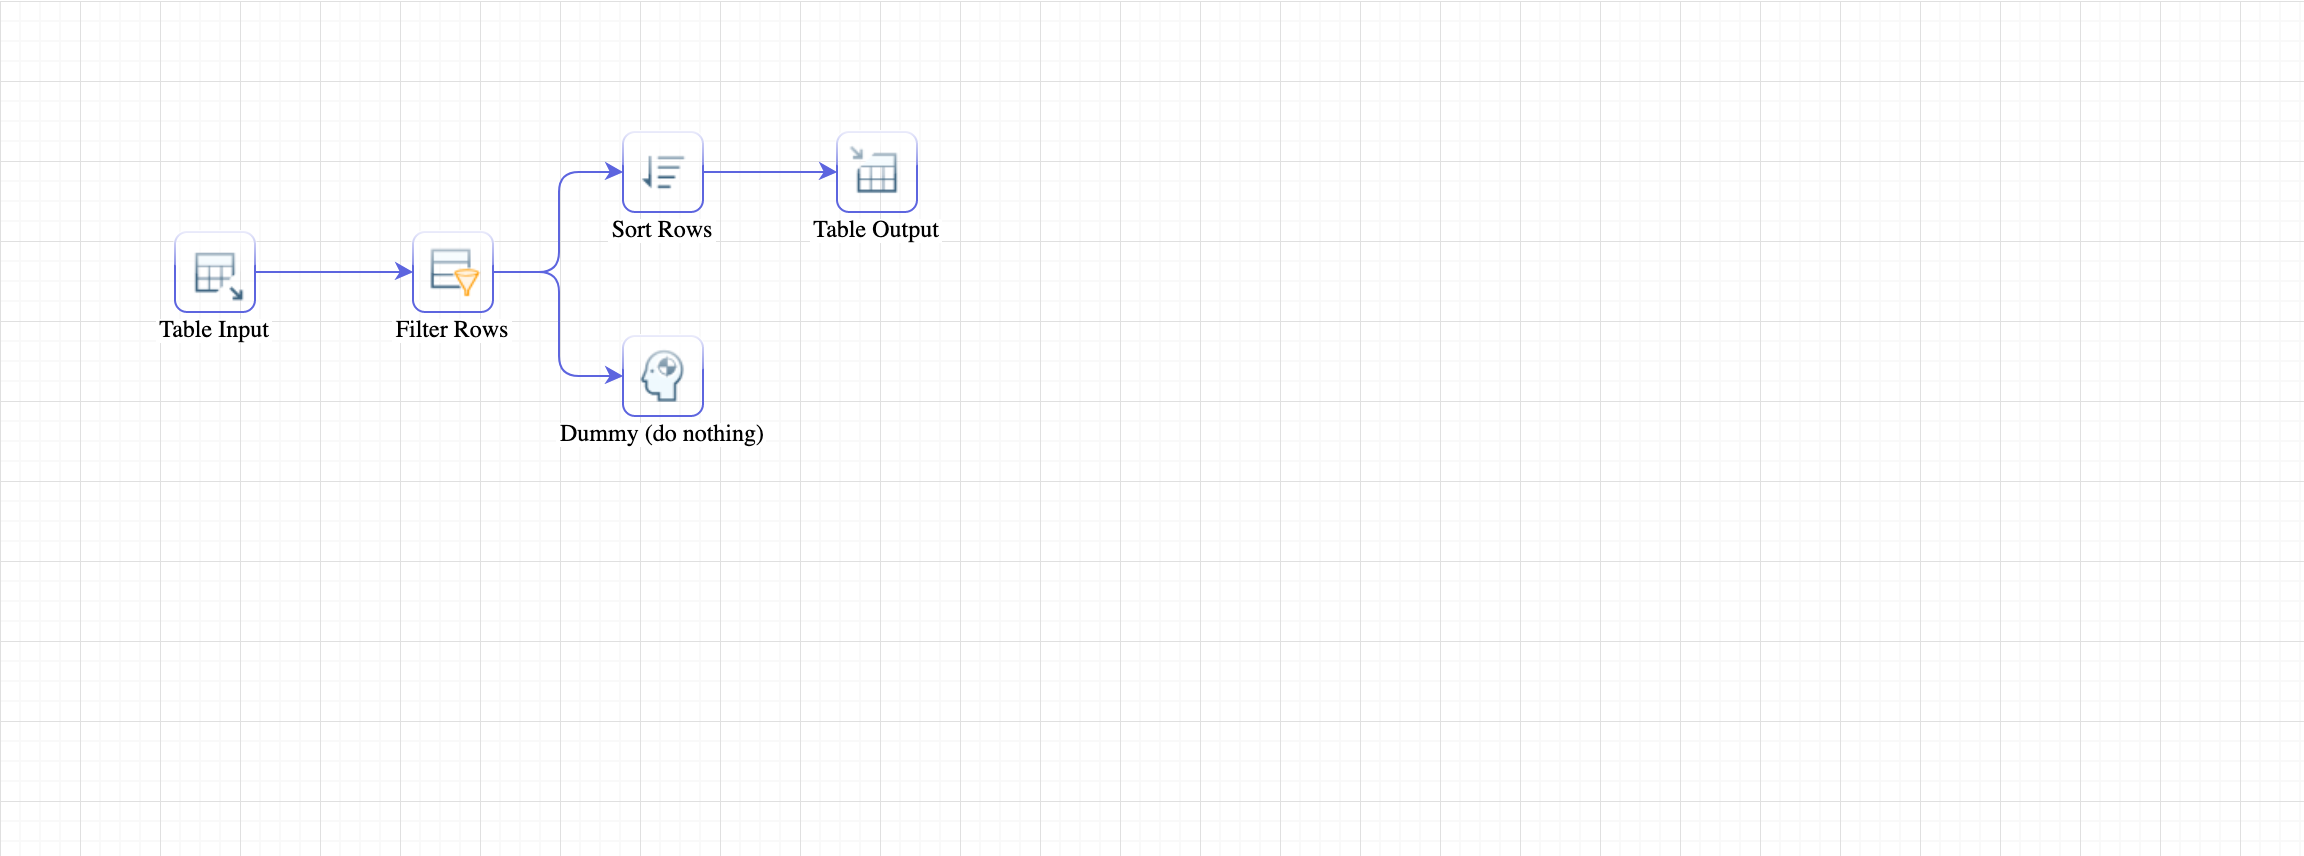
\includegraphics{images/example.png}
\caption{\label{fig:example} Simple example of an ETL pipeline represented on this editor}
\end{figure}

The components available to implement these ETL pipelines are available on the left menu. Part of this menu is represented in Figure \label{fig:components}, which is expanded the components for input, output and transformations.

\begin{figure}
\centering
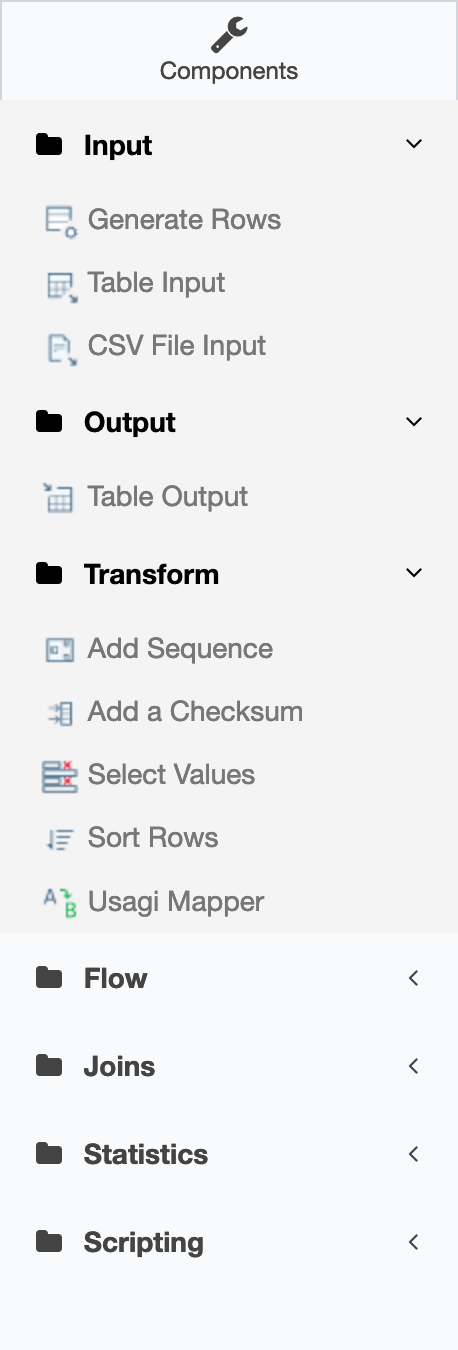
\includegraphics[width=0.25\textwidth,height=\textheight]{images/componentsOverview.png}
\caption{\label{fig:components} Overview of part of the ETL components currently deployed in the system.}
\end{figure}

The navigation bar illustrated in Figure \label{fig:navbar} allows the uses to operate over the ETL Task. This menu is divided into sub-menus: 1) step, which contains the features to configure each ETL component in the pipeline and analyse the input and output of each step; 2) execution, which defined if the ETL task will be executed locally or in a remote server; edit, contain the editing usual features, such as cut, copy, paste, delete, undo and redo; and 4) select, which is related with the drawing features.

\begin{figure}
\centering
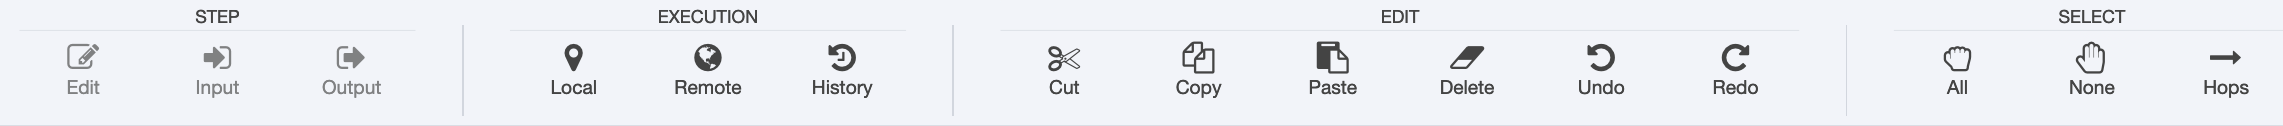
\includegraphics{images/navBarMenus.png}
\caption{\label{fig:navbar} Main features of the ETL Task Editor.}
\end{figure}

\hypertarget{guidelines-for-developers}{%
\chapter{Guidelines for Developers}\label{guidelines-for-developers}}

In this chapter, it is described the main guidelines for contributing to BIcenter.

\hypertarget{branching-convention}{%
\section{Branching Convention}\label{branching-convention}}

After some consideration, we decided to implement naming conventions in the branches being created. We followed a scheme similar to the one referred at \url{http://stackoverflow.com/a/6065944}

Each branch name is composed of the following:

\textbf{category}/\emph{name}

The possible categories are listed below.

\begin{longtable}[]{@{}
  >{\raggedright\arraybackslash}p{(\columnwidth - 2\tabcolsep) * \real{0.1042}}
  >{\raggedright\arraybackslash}p{(\columnwidth - 2\tabcolsep) * \real{0.8958}}@{}}
\toprule
\begin{minipage}[b]{\linewidth}\raggedright
Category
\end{minipage} & \begin{minipage}[b]{\linewidth}\raggedright
Description
\end{minipage} \\
\midrule
\endhead
bug & Bug fixing \\
imp & Improvement on already existing features \\
new & New features being added \\
wip & Works in progress - Big features that take long to implement and will probably hang there \\
junk & Throwaway branch created to experimentation \\
\bottomrule
\end{longtable}

The name should be concise, and directly represent what the branch solves.

Some examples:

bug/issue234

bug/fixeditdb

new/statistics

junk/tryingboostrap3

\hypertarget{adding-an-rest-api-endpoint}{%
\section{Adding an REST API endpoint}\label{adding-an-rest-api-endpoint}}

\begin{enumerate}
\def\labelenumi{\arabic{enumi}.}
\item
  Create the endpoint at \texttt{app} \textgreater{} \texttt{controllers}, either on one of the existent JAVA files or a new one if it handles a completely different topic/task, yet to be addressed.
\item
  Add the respective endpoint URL to:

  \begin{itemize}
  \tightlist
  \item
    \texttt{conf} \textgreater{} \texttt{routes}, so that the system knows that endpoint exists;
  \item
    \texttt{app} \textgreater{} \texttt{controllers} \textgreater{} \texttt{Application.java} \textgreater{} \texttt{javascriptRoutes()}, so you can use this URL dynamically at JavaScript, regarding frontend code.
  \end{itemize}
\end{enumerate}

Since the structure of this project includes both Frontend and Backend, when you create a REST API endpoint, you'll probably consume it on some frontend feature. Here's how to do that:

\begin{enumerate}
\def\labelenumi{\arabic{enumi}.}
\item
  At \texttt{app} \textgreater{} \texttt{javascripts} \textgreater{} \texttt{services}, there is a collection of JS files that have all the encapsulated logic responsible for communicating with the REST API: one file for each major entity or group of actions. So, in one of these files or a new one, add the function that handles the communication you need with the REST API through your newly developed endpoint.
\item
  At the JS controller level of your functionality, you call the function specified in the previous step with the necessary arguments and information.
\end{enumerate}

\hypertarget{example}{%
\subsection{Example}\label{example}}

This example assumes that there isn't an endpoint capable of providing information about all the existent institutions. So the purpose is to create such endpoint and provide a function that allows us to consume it on the frontend. Hence, there are 2 phases: the \textbf{creation of the REST API endpoint} and the \textbf{creation of the necessary utility to consume it} on the frontend.

\hypertarget{creation-of-rest-api-endpoint}{%
\subsubsection{Creation of REST API endpoint}\label{creation-of-rest-api-endpoint}}

Because the endpoint we want to create has the purpose of returning the information about all existent institutions, it should be placed at \texttt{app} \textgreater{} \texttt{controllers} \textgreater{} \texttt{InstitutionController.java}, with some code like this:

\begin{Shaded}
\begin{Highlighting}[]
\AttributeTok{@Security}\OperatorTok{.}\FunctionTok{Authenticated}\OperatorTok{(}\NormalTok{Secured}\OperatorTok{.}\FunctionTok{class}\OperatorTok{)}
\AttributeTok{@CheckPermission}\OperatorTok{(}\NormalTok{category }\OperatorTok{=}\NormalTok{ Category}\OperatorTok{.}\FunctionTok{INSTITUTION}\OperatorTok{,}\NormalTok{ needs }\OperatorTok{=} \OperatorTok{\{}\BuiltInTok{Operation}\OperatorTok{.}\FunctionTok{GET}\OperatorTok{\})}
\KeywordTok{public} \BuiltInTok{Result} \FunctionTok{getInstitutions}\OperatorTok{()\{}
    \BuiltInTok{String}\NormalTok{ email }\OperatorTok{=} \FunctionTok{session}\OperatorTok{().}\FunctionTok{get}\OperatorTok{(}\StringTok{"userEmail"}\OperatorTok{);}
    \BuiltInTok{List}\OperatorTok{\textless{}}\NormalTok{Institution}\OperatorTok{\textgreater{}}\NormalTok{ institutions }\OperatorTok{=}\NormalTok{ institutionRepository}\OperatorTok{.}\FunctionTok{list}\OperatorTok{(}\NormalTok{email}\OperatorTok{);}

\NormalTok{    ObjectMapper mapper }\OperatorTok{=} \KeywordTok{new} \FunctionTok{ObjectMapper}\OperatorTok{();}
\NormalTok{    SimpleModule module }\OperatorTok{=} \KeywordTok{new} \FunctionTok{SimpleModule}\OperatorTok{();}
\NormalTok{    module}\OperatorTok{.}\FunctionTok{addSerializer}\OperatorTok{(}\NormalTok{Institution}\OperatorTok{.}\FunctionTok{class}\OperatorTok{,} \KeywordTok{new} \FunctionTok{InstitutionSerializer}\OperatorTok{());}
\NormalTok{    module}\OperatorTok{.}\FunctionTok{addSerializer}\OperatorTok{(}\NormalTok{Task}\OperatorTok{.}\FunctionTok{class}\OperatorTok{,} \KeywordTok{new} \FunctionTok{SimpleTaskSerializer}\OperatorTok{());}
\NormalTok{    module}\OperatorTok{.}\FunctionTok{addSerializer}\OperatorTok{(}\NormalTok{Server}\OperatorTok{.}\FunctionTok{class}\OperatorTok{,} \KeywordTok{new} \FunctionTok{ServerSerializer}\OperatorTok{());}
\NormalTok{    module}\OperatorTok{.}\FunctionTok{addSerializer}\OperatorTok{(}\BuiltInTok{DataSource}\OperatorTok{.}\FunctionTok{class}\OperatorTok{,} \KeywordTok{new} \FunctionTok{DataSourceSerializer}\OperatorTok{());}
\NormalTok{    mapper}\OperatorTok{.}\FunctionTok{registerModule}\OperatorTok{(}\NormalTok{module}\OperatorTok{);}
\NormalTok{    Json}\OperatorTok{.}\FunctionTok{setObjectMapper}\OperatorTok{(}\NormalTok{mapper}\OperatorTok{);}

    \ControlFlowTok{return} \FunctionTok{ok}\OperatorTok{(}\NormalTok{Json}\OperatorTok{.}\FunctionTok{toJson}\OperatorTok{(}\NormalTok{institutions}\OperatorTok{));}
\OperatorTok{\}}
\end{Highlighting}
\end{Shaded}

After creating the endpoint, we need to make it discoverable (be available to the outside world). To do that, we add its URL to:
1. \texttt{conf} \textgreater{} \texttt{routes}:

\begin{Shaded}
\begin{Highlighting}[]
\NormalTok{...}
\NormalTok{GET          /institution/list                    controllers.InstitutionController.getInstitutions()}
\NormalTok{...}
\end{Highlighting}
\end{Shaded}

\begin{enumerate}
\def\labelenumi{\arabic{enumi}.}
\setcounter{enumi}{1}
\tightlist
\item
  \texttt{app} \textgreater{} \texttt{controllers} \textgreater{} \texttt{Application.java} \textgreater{} \texttt{javascriptRoutes()}:
\end{enumerate}

\begin{Shaded}
\begin{Highlighting}[]
\KeywordTok{public} \BuiltInTok{Result} \FunctionTok{javascriptRoutes}\OperatorTok{()} \OperatorTok{\{}
    \FunctionTok{response}\OperatorTok{().}\FunctionTok{setHeader}\OperatorTok{(}\NormalTok{Http}\OperatorTok{.}\FunctionTok{HeaderNames}\OperatorTok{.}\FunctionTok{CONTENT\_TYPE}\OperatorTok{,} \StringTok{"text/javascript"}\OperatorTok{);}
    \ControlFlowTok{return} \FunctionTok{ok}\OperatorTok{(}\NormalTok{JavaScriptReverseRouter}\OperatorTok{.}\FunctionTok{create}\OperatorTok{(}\StringTok{"jsRoutes"}\OperatorTok{,}
        \KeywordTok{...}\OperatorTok{,}

\NormalTok{        routes}\OperatorTok{.}\FunctionTok{javascript}\OperatorTok{.}\FunctionTok{InstitutionController}\OperatorTok{.}\FunctionTok{getInstitutions}\OperatorTok{(),}

        \KeywordTok{...}
    \OperatorTok{));}
\OperatorTok{\}}
\end{Highlighting}
\end{Shaded}

\hypertarget{creation-of-utility-function-to-consume-the-rest-endpoint}{%
\subsubsection{Creation of utility function to consume the REST endpoint}\label{creation-of-utility-function-to-consume-the-rest-endpoint}}

This second phase explains how to create the referred utility function so we can more easily consume the developed endpoint. Since it's an institution-related method, we will be adding the following utility function to \texttt{app} \textgreater{} \texttt{javascripts} \textgreater{} \texttt{services} \textgreater{} \texttt{institution.js}.

\begin{Shaded}
\begin{Highlighting}[]
\NormalTok{Institution}\OperatorTok{.}\AttributeTok{getInstitutions} \OperatorTok{=} \KeywordTok{function}\NormalTok{ (callback) \{}
\NormalTok{    jsRoutes}\OperatorTok{.}\AttributeTok{controllers}\OperatorTok{.}\AttributeTok{InstitutionController}\OperatorTok{.}\FunctionTok{getInstitutions}\NormalTok{()}\OperatorTok{.}\FunctionTok{ajax}\NormalTok{(\{}
    \DataTypeTok{contentType}\OperatorTok{:} \StringTok{\textquotesingle{}application/json; charset=utf{-}8\textquotesingle{}}\OperatorTok{,}
        \DataTypeTok{success}\OperatorTok{:} \KeywordTok{function}\NormalTok{ (response) \{}
            \ControlFlowTok{if}\NormalTok{ (callback) \{}
                \FunctionTok{callback}\NormalTok{(response)}\OperatorTok{;}
\NormalTok{            \}}
\NormalTok{        \}}\OperatorTok{,}
        \DataTypeTok{error}\OperatorTok{:} \KeywordTok{function}\NormalTok{ (response) \{}
            \BuiltInTok{console}\OperatorTok{.}\FunctionTok{error}\NormalTok{(}\StringTok{\textquotesingle{}Error in Institution service\textquotesingle{}}\OperatorTok{,}\NormalTok{ response)}\OperatorTok{;}
\NormalTok{        \}}
\NormalTok{    \})}
\NormalTok{ \}}\OperatorTok{;}
\end{Highlighting}
\end{Shaded}

This consumes the endpoint and, on success calls the specified callback function; otherwise (on fail) displays an error message on your browser's console.

After this, the final part is to consume this utility function, which can also be called a service. A simple example is to use the service on your javascript file that bears the ``backend'' responsibility of your UI component/view, in a similar way to the following code:

\begin{Shaded}
\begin{Highlighting}[]
\NormalTok{Institution}\OperatorTok{.}\FunctionTok{getInstitutions}\NormalTok{(}\KeywordTok{function}\NormalTok{ (institutions) \{}
    \CommentTok{// do whatever you need with the returned information}
\NormalTok{\})}\OperatorTok{;}
\end{Highlighting}
\end{Shaded}

\hypertarget{adding-web-view}{%
\section{Adding web view}\label{adding-web-view}}

If you want to create an entirely new base schema (a view), you first need to add a base template name \texttt{\textless{}name\textgreater{}.scala.html} to \texttt{app} \textgreater{} \texttt{views}. You also need to make sure that you have an endpoint on JAVA code that handles your request and returns this web view (the ``\textbf{backend}'' process is similar to create a REST API endpoint).

If you just want to create a new UI stage, based on an already defined view, follow these steps:
1. Create an endpoint (and register it) that returns the base view you want to use.

\begin{enumerate}
\def\labelenumi{\arabic{enumi}.}
\setcounter{enumi}{1}
\item
  At \texttt{app} \textgreater{} \texttt{assets} \textgreater{} \texttt{javascripts}, create the controller and view associated with your new UI stage (the view JS file handles the stuff UI related and the controller handles the stuff Backend related).
\item
  At \texttt{app} \textgreater{} \texttt{assets} \textgreater{} \texttt{templates}, create a file named \texttt{\textless{}name\textgreater{}.handlebars} where you'll insert the UI code that will be dynamically added to the main div container of your base web view.
\item
  After all these files are ready, you need to make sure the framework knows the path to everything you created, so you'll need to add the paths to your view and controller javascript files in the file \texttt{app} \textgreater{} \texttt{assets} \textgreater{} \texttt{javacripts} \textgreater{} \texttt{main.js}.
\item
  Finally, you'll need to add the RegExp handler that will assemble the resources you need (variables and controllers) at \texttt{app} \textgreater{} \texttt{assets} \textgreater{} \texttt{application} \textgreater{} \texttt{application.js}.
\end{enumerate}

\hypertarget{example-1}{%
\subsection{Example}\label{example-1}}

This example is going to be divided into two big parts: the \textbf{creation of a new view from scratch} and the \textbf{creation of a UI component} (through handlebars).

Let's take as an example the creation of a dashboard page, given the fact that we need to create a new base-view from scratch.

\textbf{NOTE:} if you just want to create a new UI component, with handlebars, jump to the second part.

\hypertarget{creation-of-a-new-base-view}{%
\subsection{Creation of a new (base) view}\label{creation-of-a-new-base-view}}

To create a new view to use as a base to new UI stages, you first need to add the HTML template. So, add your view structure to a file named \texttt{home.scala.html}, for the sake of this example, at \texttt{app} \textgreater{} \texttt{views}:

\begin{Shaded}
\begin{Highlighting}[]
\DataTypeTok{\textless{}!DOCTYPE }\NormalTok{html}\DataTypeTok{\textgreater{}}

\KeywordTok{\textless{}html\textgreater{}}
    \KeywordTok{\textless{}head\textgreater{}}
        \KeywordTok{\textless{}meta} \ErrorTok{charset}\OtherTok{=}\StringTok{"UTF{-}8"}\KeywordTok{\textgreater{}}
    \KeywordTok{\textless{}meta} \ErrorTok{http{-}equiv}\OtherTok{=}\StringTok{"X{-}UA{-}Compatible"} \ErrorTok{content}\OtherTok{=}\StringTok{"IE=edge"}\KeywordTok{\textgreater{}}
    \CommentTok{\textless{}!{-}{-} Tell the browser to be responsive to screen width {-}{-}\textgreater{}}
    \KeywordTok{\textless{}meta} \ErrorTok{content}\OtherTok{=}\StringTok{"width=device{-}width, initial{-}scale=1, maximum{-}scale=1, user{-}scalable=no"} \ErrorTok{name}\OtherTok{=}\StringTok{"viewport"}\KeywordTok{\textgreater{}}

    \KeywordTok{\textless{}title\textgreater{}}\NormalTok{BIcenter}\KeywordTok{\textless{}/title\textgreater{}}

    \CommentTok{\textless{}!{-}{-} Boostrap Select2 {-}{-}\textgreater{}}
    \KeywordTok{\textless{}link} \ErrorTok{rel}\OtherTok{=}\StringTok{"stylesheet"} \ErrorTok{media}\OtherTok{=}\StringTok{"screen"} \ErrorTok{href}\OtherTok{=}\StringTok{"@routes.Assets.versioned("}\ErrorTok{lib/select2/select2.min.css")"}\KeywordTok{\textgreater{}}

    \CommentTok{\textless{}!{-}{-} Font Awesome {-}{-}\textgreater{}}
    \KeywordTok{\textless{}link} \ErrorTok{rel}\OtherTok{=}\StringTok{"stylesheet"} \ErrorTok{media}\OtherTok{=}\StringTok{"screen"} \ErrorTok{href}\OtherTok{=}\StringTok{"@routes.Assets.versioned("}\ErrorTok{lib/font{-}awesome/css/font{-}awesome.min.css")"}\KeywordTok{\textgreater{}}
    \CommentTok{\textless{}!{-}{-} PNotify {-}{-}\textgreater{}}
    \KeywordTok{\textless{}link} \ErrorTok{rel}\OtherTok{=}\StringTok{"stylesheet"} \ErrorTok{media}\OtherTok{=}\StringTok{"screen"} \ErrorTok{href}\OtherTok{=}\StringTok{"@routes.Assets.versioned("}\ErrorTok{lib/pnotify/pnotify.css")"}\KeywordTok{\textgreater{}}
    \KeywordTok{\textless{}link} \ErrorTok{rel}\OtherTok{=}\StringTok{"stylesheet"} \ErrorTok{media}\OtherTok{=}\StringTok{"screen"} \ErrorTok{href}\OtherTok{=}\StringTok{"@routes.Assets.versioned("}\ErrorTok{lib/pnotify/pnotify.nonblock.css")"}\KeywordTok{\textgreater{}}
    \CommentTok{\textless{}!{-}{-} query{-}builder {-}{-}\textgreater{}}
    \KeywordTok{\textless{}link} \ErrorTok{rel}\OtherTok{=}\StringTok{"stylesheet"} \ErrorTok{media}\OtherTok{=}\StringTok{"screen"} \ErrorTok{href}\OtherTok{=}\StringTok{"@routes.Assets.versioned("}\ErrorTok{lib/jQuery{-}QueryBuilder/css/query{-}builder.default.min.css")"}\KeywordTok{\textgreater{}}

    \KeywordTok{\textless{}link} \ErrorTok{rel}\OtherTok{=}\StringTok{"shortcut icon"} \ErrorTok{type}\OtherTok{=}\StringTok{"image/png"} \ErrorTok{href}\OtherTok{=}\StringTok{"@routes.Assets.versioned("}\ErrorTok{images/favicon.png")"}\KeywordTok{\textgreater{}}

    \CommentTok{\textless{}!{-}{-}DataTable dependencies {-}{-}\textgreater{}}
    \KeywordTok{\textless{}link} \ErrorTok{rel}\OtherTok{=}\StringTok{"stylesheet"} \ErrorTok{media}\OtherTok{=}\StringTok{"screen"} \ErrorTok{href}\OtherTok{=}\StringTok{"@routes.Assets.versioned("}\ErrorTok{lib/datatables/dataTables.bootstrap.min.css")"}\KeywordTok{\textgreater{}}
    \KeywordTok{\textless{}link} \ErrorTok{rel}\OtherTok{=}\StringTok{"stylesheet"} \ErrorTok{media}\OtherTok{=}\StringTok{"screen"} \ErrorTok{href}\OtherTok{=}\StringTok{"@routes.Assets.versioned("}\ErrorTok{lib/datatables/buttons.dataTables.min.css")"}\KeywordTok{\textgreater{}}

    \CommentTok{\textless{}!{-}{-} jQuery UI {-}{-}\textgreater{}}
    \KeywordTok{\textless{}link} \ErrorTok{rel}\OtherTok{=}\StringTok{"stylesheet"} \ErrorTok{media}\OtherTok{=}\StringTok{"screen"} \ErrorTok{href}\OtherTok{=}\StringTok{"@routes.Assets.versioned("}\ErrorTok{lib/jquery{-}ui/jquery{-}ui.css")"}\KeywordTok{\textgreater{}}

    \CommentTok{\textless{}!{-}{-} Boostrap DateTime{-}Picker {-}{-}\textgreater{}}
    \KeywordTok{\textless{}link} \ErrorTok{rel}\OtherTok{=}\StringTok{"stylesheet"} \ErrorTok{media}\OtherTok{=}\StringTok{"screen"} \ErrorTok{href}\OtherTok{=}\StringTok{"@routes.Assets.versioned("}\ErrorTok{lib/bootstrap{-}datetimepicker/bootstrap{-}datetimepicker.min.css")"}\KeywordTok{\textgreater{}}

    \CommentTok{\textless{}!{-}{-} iCheck {-}{-}\textgreater{}}
    \KeywordTok{\textless{}link} \ErrorTok{rel}\OtherTok{=}\StringTok{"stylesheet"} \ErrorTok{media}\OtherTok{=}\StringTok{"screen"} \ErrorTok{href}\OtherTok{=}\StringTok{"@routes.Assets.versioned("}\ErrorTok{lib/iCheck/all.css")"}\KeywordTok{\textgreater{}}
    \KeywordTok{\textless{}link} \ErrorTok{rel}\OtherTok{=}\StringTok{"stylesheet"} \ErrorTok{media}\OtherTok{=}\StringTok{"screen"} \ErrorTok{href}\OtherTok{=}\StringTok{"@routes.Assets.versioned("}\ErrorTok{lib/iCheck/square/blue.css")"}\KeywordTok{\textgreater{}}

    \CommentTok{\textless{}!{-}{-} Main CSS: Bootstrap + AdminLTE + Custom css {-}{-}\textgreater{}}
    \KeywordTok{\textless{}link} \ErrorTok{rel}\OtherTok{=}\StringTok{"stylesheet"} \ErrorTok{media}\OtherTok{=}\StringTok{"screen"} \ErrorTok{href}\OtherTok{=}\StringTok{"@routes.Assets.versioned("}\ErrorTok{stylesheets/main.min.css")"}\KeywordTok{\textgreater{}}
    \KeywordTok{\textless{}/head\textgreater{}}
    \KeywordTok{\textless{}body} \ErrorTok{style}\OtherTok{=}\StringTok{"height:auto;"} \ErrorTok{class}\OtherTok{=}\StringTok{"skin{-}darkblue{-}light fixed home{-}page"}\KeywordTok{\textgreater{}}
        \KeywordTok{\textless{}script}\OtherTok{ type=}\StringTok{"text/javascript"} \ErrorTok{src}\OtherTok{=}\StringTok{"@routes.Assets.versioned("}\ErrorTok{lib/mxgraph2/js/mxClient.js")"}\KeywordTok{\textgreater{}\textless{}/script\textgreater{}}
    \KeywordTok{\textless{}script}\OtherTok{ type=}\StringTok{"text/javascript"} \ErrorTok{src}\OtherTok{=}\StringTok{"@routes.Assets.versioned("}\ErrorTok{editor/editor.js")"}\KeywordTok{\textgreater{}\textless{}/script\textgreater{}}
    \KeywordTok{\textless{}script}\OtherTok{ type=}\StringTok{"text/javascript"} \ErrorTok{src}\OtherTok{=}\StringTok{"@routes.Assets.versioned("}\ErrorTok{editor/graph.js")"}\KeywordTok{\textgreater{}\textless{}/script\textgreater{}}

    \KeywordTok{\textless{}div} \ErrorTok{class}\OtherTok{=}\StringTok{"container"}\KeywordTok{\textgreater{}}
        \KeywordTok{\textless{}div} \ErrorTok{module}\OtherTok{=}\StringTok{"HeaderModule"}\KeywordTok{\textgreater{}}
\NormalTok{            @header()}
        \KeywordTok{\textless{}/div\textgreater{}}

        \KeywordTok{\textless{}div} \ErrorTok{module}\OtherTok{=}\StringTok{"MainModule"}\KeywordTok{\textgreater{}}
            \KeywordTok{\textless{}div} \ErrorTok{controller}\OtherTok{=}\StringTok{"HomeController"}\KeywordTok{\textgreater{}\textless{}/div\textgreater{}}
        \KeywordTok{\textless{}/div\textgreater{}}

        \KeywordTok{\textless{}div} \ErrorTok{class}\OtherTok{=}\StringTok{"navbar{-}fixed{-}bottom"}\KeywordTok{\textgreater{}}
\NormalTok{            @footer()}
        \KeywordTok{\textless{}/div\textgreater{}}
        \KeywordTok{\textless{}/div\textgreater{}}

        \KeywordTok{\textless{}script}\OtherTok{ type=}\StringTok{"text/javascript"} \ErrorTok{data{-}main}\OtherTok{=}\StringTok{"@routes.Assets.versioned("}\ErrorTok{javascripts/main")"} \ErrorTok{src}\OtherTok{=}\StringTok{"@routes.Assets.versioned("}\ErrorTok{lib/requirejs/require.min.js")"}\KeywordTok{\textgreater{}\textless{}/script\textgreater{}}
    \KeywordTok{\textless{}/body\textgreater{}}
\KeywordTok{\textless{}/html\textgreater{}}
\end{Highlighting}
\end{Shaded}

After creating the template, you now need to create an endpoint to return this view and register it in the system.

So, to create the endpoint you add a new controller at \texttt{app} \textgreater{} \texttt{controllers} or add a function to an existent controller. In this example we will create a new controller called \texttt{HomeController.java}:

\begin{Shaded}
\begin{Highlighting}[]
\KeywordTok{public} \KeywordTok{class}\NormalTok{ HomeController }\KeywordTok{extends}\NormalTok{ Controller }\OperatorTok{\{}
    \AttributeTok{@Security}\OperatorTok{.}\FunctionTok{Authenticated}\OperatorTok{(}\NormalTok{Secured}\OperatorTok{.}\FunctionTok{class}\OperatorTok{)}
    \KeywordTok{public} \BuiltInTok{Result} \FunctionTok{index}\OperatorTok{()} \OperatorTok{\{}
        \ControlFlowTok{return} \FunctionTok{ok}\OperatorTok{(}\NormalTok{views}\OperatorTok{.}\FunctionTok{html}\OperatorTok{.}\FunctionTok{home}\OperatorTok{.}\FunctionTok{render}\OperatorTok{());}
    \OperatorTok{\}}
\OperatorTok{\}}
\end{Highlighting}
\end{Shaded}

And, then, to register it, add to:
1. \texttt{conf} \textgreater{} \texttt{routes}:

\begin{Shaded}
\begin{Highlighting}[]
\NormalTok{...}

\NormalTok{GET               /home                    controllers.HomeController.index()}

\NormalTok{...}
\end{Highlighting}
\end{Shaded}

\begin{enumerate}
\def\labelenumi{\arabic{enumi}.}
\setcounter{enumi}{1}
\tightlist
\item
  \texttt{app} \textgreater{} \texttt{controllers} \textgreater{} \texttt{Application.java} \textgreater{} \texttt{javascriptRoutes()}:
\end{enumerate}

\begin{Shaded}
\begin{Highlighting}[]
\KeywordTok{public} \BuiltInTok{Result} \FunctionTok{javascriptRoutes}\OperatorTok{()} \OperatorTok{\{}
    \FunctionTok{response}\OperatorTok{().}\FunctionTok{setHeader}\OperatorTok{(}\NormalTok{Http}\OperatorTok{.}\FunctionTok{HeaderNames}\OperatorTok{.}\FunctionTok{CONTENT\_TYPE}\OperatorTok{,} \StringTok{"text/javascript"}\OperatorTok{);}
    \ControlFlowTok{return} \FunctionTok{ok}\OperatorTok{(}\NormalTok{JavaScriptReverseRouter}\OperatorTok{.}\FunctionTok{create}\OperatorTok{(}\StringTok{"jsRoutes"}\OperatorTok{,}
        \KeywordTok{...}\OperatorTok{,}

\NormalTok{        routes}\OperatorTok{.}\FunctionTok{javascript}\OperatorTok{.}\FunctionTok{HomeController}\OperatorTok{.}\FunctionTok{index}\OperatorTok{(),}

        \KeywordTok{...}
    \OperatorTok{));}
\OperatorTok{\}}
\end{Highlighting}
\end{Shaded}

\hypertarget{creation-of-a-ui-component-handlebars}{%
\subsection{Creation of a UI component (handlebars)}\label{creation-of-a-ui-component-handlebars}}

Once the URL for the base view is configured, the next step is to create the functional files that handle frontend and backend of the UI element. So, we will create a folder \texttt{home} at \texttt{app} \textgreater{} \texttt{assets} \textgreater{} \texttt{javascripts}. Inside this folder create tho files: \texttt{homeController.js} and \texttt{homeView.js}.

The \texttt{homeController.js} is responsible to handle the backend operations and should follow a structure similar to this:

\begin{Shaded}
\begin{Highlighting}[]
\FunctionTok{define}\NormalTok{(}\StringTok{\textquotesingle{}HomeController\textquotesingle{}}\OperatorTok{,}\NormalTok{ [}\StringTok{\textquotesingle{}Controller\textquotesingle{}}\OperatorTok{,} \StringTok{\textquotesingle{}HomeView\textquotesingle{}}\OperatorTok{,} \StringTok{\textquotesingle{}Router\textquotesingle{}}\OperatorTok{,} \StringTok{\textquotesingle{}Institution\textquotesingle{}}\OperatorTok{,} \StringTok{\textquotesingle{}Task\textquotesingle{}}\OperatorTok{,} \StringTok{\textquotesingle{}Alert\textquotesingle{}}\OperatorTok{,} \StringTok{\textquotesingle{}jquery\textquotesingle{}}\OperatorTok{,} \StringTok{\textquotesingle{}jsRoutes\textquotesingle{}}\OperatorTok{,} \StringTok{\textquotesingle{}jquery{-}cookie\textquotesingle{}}\NormalTok{]}\OperatorTok{,} \KeywordTok{function}\NormalTok{ (Controller}\OperatorTok{,}\NormalTok{ HomeView}\OperatorTok{,}\NormalTok{ Router}\OperatorTok{,}\NormalTok{ Institution}\OperatorTok{,}\NormalTok{ Task}\OperatorTok{,}\NormalTok{ Alert}\OperatorTok{,}\NormalTok{ $}\OperatorTok{,}\NormalTok{ jsRoutes) \{}
    \KeywordTok{const}\NormalTok{ HomeController }\OperatorTok{=} \KeywordTok{function}\NormalTok{ (module) \{}
\NormalTok{        Controller}\OperatorTok{.}\FunctionTok{call}\NormalTok{(}\KeywordTok{this}\OperatorTok{,}\NormalTok{ module}\OperatorTok{,} \KeywordTok{new} \FunctionTok{HomeView}\NormalTok{(}\KeywordTok{this}\NormalTok{))}\OperatorTok{;}
\NormalTok{    \}}\OperatorTok{;}

    \CommentTok{// Inheritance from the superclass}
\NormalTok{    HomeController}\OperatorTok{.}\AttributeTok{prototype} \OperatorTok{=} \BuiltInTok{Object}\OperatorTok{.}\FunctionTok{create}\NormalTok{(Controller}\OperatorTok{.}\AttributeTok{prototype}\NormalTok{)}\OperatorTok{;}
    \KeywordTok{const}\NormalTok{ \_super\_ }\OperatorTok{=}\NormalTok{ Controller}\OperatorTok{.}\AttributeTok{prototype}\OperatorTok{;}

\NormalTok{    HomeController}\OperatorTok{.}\AttributeTok{prototype}\OperatorTok{.}\AttributeTok{initialize} \OperatorTok{=} \KeywordTok{function}\NormalTok{ ($container) \{}
\NormalTok{        \_super\_}\OperatorTok{.}\AttributeTok{initialize}\OperatorTok{.}\FunctionTok{call}\NormalTok{(}\KeywordTok{this}\OperatorTok{,}\NormalTok{ $container)}\OperatorTok{;}

    \KeywordTok{this}\OperatorTok{.}\FunctionTok{getTasks}\NormalTok{()}\OperatorTok{;}
\NormalTok{    \}}\OperatorTok{;}

\NormalTok{    HomeController}\OperatorTok{.}\AttributeTok{prototype}\OperatorTok{.}\AttributeTok{getTasks} \OperatorTok{=} \KeywordTok{function}\NormalTok{ () \{}
        \KeywordTok{const}\NormalTok{ context }\OperatorTok{=} \KeywordTok{this}\OperatorTok{;}
\NormalTok{    Institution}\OperatorTok{.}\FunctionTok{getInstitutions}\NormalTok{(}\KeywordTok{function}\NormalTok{ (institutions) \{}
\NormalTok{        context}\OperatorTok{.}\AttributeTok{view}\OperatorTok{.}\FunctionTok{loadInstitutions}\NormalTok{(institutions)}\OperatorTok{;}
\NormalTok{    \})}\OperatorTok{;}
\NormalTok{    \}}\OperatorTok{;}

    \ControlFlowTok{return}\NormalTok{ HomeController}\OperatorTok{;}
\NormalTok{\})}\OperatorTok{;}
\end{Highlighting}
\end{Shaded}

On the other hand, the \texttt{homeView.js}is responsible for frontend interactions and should follow a structure similar to:

\begin{Shaded}
\begin{Highlighting}[]
\FunctionTok{define}\NormalTok{(}\StringTok{\textquotesingle{}HomeView\textquotesingle{}}\OperatorTok{,}\NormalTok{ [}\StringTok{\textquotesingle{}jquery\textquotesingle{}}\OperatorTok{,} \StringTok{\textquotesingle{}View\textquotesingle{}}\NormalTok{]}\OperatorTok{,} \KeywordTok{function}\NormalTok{ ($}\OperatorTok{,}\NormalTok{ View) \{}
    \KeywordTok{const}\NormalTok{ HomeView }\OperatorTok{=} \KeywordTok{function}\NormalTok{ (controller) \{}
\NormalTok{        View}\OperatorTok{.}\FunctionTok{call}\NormalTok{(}\KeywordTok{this}\OperatorTok{,}\NormalTok{ controller}\OperatorTok{,} \StringTok{\textquotesingle{}home\textquotesingle{}}\NormalTok{)}\OperatorTok{;}
\NormalTok{    \}}\OperatorTok{;}

    \CommentTok{// Inheritance from super class}
\NormalTok{    HomeView}\OperatorTok{.}\AttributeTok{prototype} \OperatorTok{=} \BuiltInTok{Object}\OperatorTok{.}\FunctionTok{create}\NormalTok{(View}\OperatorTok{.}\AttributeTok{prototype}\NormalTok{)}\OperatorTok{;}
    \KeywordTok{const}\NormalTok{ \_super\_ }\OperatorTok{=}\NormalTok{ View}\OperatorTok{.}\AttributeTok{prototype}\OperatorTok{;}

\NormalTok{    HomeView}\OperatorTok{.}\AttributeTok{prototype}\OperatorTok{.}\AttributeTok{initialize} \OperatorTok{=} \KeywordTok{function}\NormalTok{ ($container) \{}
\NormalTok{        \_super\_}\OperatorTok{.}\AttributeTok{initialize}\OperatorTok{.}\FunctionTok{call}\NormalTok{(}\KeywordTok{this}\OperatorTok{,}\NormalTok{ $container)}\OperatorTok{;}
\NormalTok{    \}}\OperatorTok{;}

\NormalTok{    HomeView}\OperatorTok{.}\AttributeTok{prototype}\OperatorTok{.}\AttributeTok{loadInstitutions} \OperatorTok{=} \KeywordTok{function}\NormalTok{ (institutions) \{}
        \KeywordTok{const}\NormalTok{ html }\OperatorTok{=}\NormalTok{ JST[}\StringTok{\textquotesingle{}home\textquotesingle{}}\NormalTok{](\{}
        \DataTypeTok{institutions}\OperatorTok{:}\NormalTok{ institutions}
\NormalTok{        \})}\OperatorTok{;}
        \KeywordTok{this}\OperatorTok{.}\AttributeTok{$container}\OperatorTok{.}\FunctionTok{html}\NormalTok{(html)}\OperatorTok{;}
    \KeywordTok{this}\OperatorTok{.}\FunctionTok{\_loadViewComponents}\NormalTok{()}\OperatorTok{;}
\NormalTok{    \}}\OperatorTok{;}

    \ControlFlowTok{return}\NormalTok{ HomeView}\OperatorTok{;}
\NormalTok{\})}\OperatorTok{;}
\end{Highlighting}
\end{Shaded}

As can be seen in this last code snippet, we ``import'' a web (HTML) structure from \texttt{\textquotesingle{}home\textquotesingle{}}. This refers to the file \texttt{home.handlebars} that must be placed at \texttt{app} \textgreater{} \texttt{assets} \textgreater{} \texttt{templates}. Hence, we will create this exact file in the specified location with the following content:

\begin{Shaded}
\begin{Highlighting}[]
\KeywordTok{\textless{}div} \ErrorTok{class}\OtherTok{=}\StringTok{"main{-}div"}\KeywordTok{\textgreater{}}
    \KeywordTok{\textless{}div} \ErrorTok{class}\OtherTok{=}\StringTok{"title"}\KeywordTok{\textgreater{}}
        \KeywordTok{\textless{}h1\textgreater{}\textless{}b\textgreater{}\textless{}i} \ErrorTok{class}\OtherTok{=}\StringTok{"fa fa{-}hospital{-}o"}\KeywordTok{\textgreater{}\textless{}/i\textgreater{}}\NormalTok{ Dashboard: Resources}\KeywordTok{\textless{}/b\textgreater{}\textless{}/h1\textgreater{}}
    \KeywordTok{\textless{}/div\textgreater{}}

    \KeywordTok{\textless{}div} \ErrorTok{id}\OtherTok{=}\StringTok{"institutions"} \ErrorTok{view{-}element}\OtherTok{=}\StringTok{"institutions"} \ErrorTok{class}\OtherTok{=}\StringTok{"row"}\KeywordTok{\textgreater{}}
\NormalTok{        \{\{\#institutions\}\}}
            \KeywordTok{\textless{}div} \ErrorTok{class}\OtherTok{=}\StringTok{"institution col{-}lg{-}4"}\KeywordTok{\textgreater{}}
                \KeywordTok{\textless{}div} \ErrorTok{class}\OtherTok{=}\StringTok{"panel panel{-}default"}\KeywordTok{\textgreater{}}
                    \KeywordTok{\textless{}div} \ErrorTok{class}\OtherTok{=}\StringTok{"panel{-}heading"}\KeywordTok{\textgreater{}}
                        \KeywordTok{\textless{}h3} \ErrorTok{class}\OtherTok{=}\StringTok{"panel{-}title"}\KeywordTok{\textgreater{}\textless{}b\textgreater{}}\NormalTok{\{\{name\}\}}\KeywordTok{\textless{}/b\textgreater{}\textless{}/h3\textgreater{}}
                    \KeywordTok{\textless{}/div\textgreater{}}
                    \KeywordTok{\textless{}div} \ErrorTok{class}\OtherTok{=}\StringTok{"panel{-}body"}\KeywordTok{\textgreater{}}
                        \KeywordTok{\textless{}ul} \ErrorTok{class}\OtherTok{=}\StringTok{"treeview{-}menu"} \ErrorTok{data{-}widget}\OtherTok{=}\StringTok{"tree"}\KeywordTok{\textgreater{}}
                            \CommentTok{\textless{}!{-}{-} Tasks {-}{-}\textgreater{}}
                            \KeywordTok{\textless{}li} \ErrorTok{class}\OtherTok{=}\StringTok{"treeview menu"}\KeywordTok{\textgreater{}}
                                \KeywordTok{\textless{}a} \ErrorTok{name}\OtherTok{=}\StringTok{"tasks"}\KeywordTok{\textgreater{}}
                                    \KeywordTok{\textless{}i} \ErrorTok{class}\OtherTok{=}\StringTok{"fa fa{-}folder"}\KeywordTok{\textgreater{}\textless{}/i\textgreater{}} \KeywordTok{\textless{}span\textgreater{}}\NormalTok{Tasks}\KeywordTok{\textless{}/span\textgreater{}}
                                    \KeywordTok{\textless{}span} \ErrorTok{class}\OtherTok{=}\StringTok{"pull{-}right{-}container"}\KeywordTok{\textgreater{}}
                                    \KeywordTok{\textless{}i} \ErrorTok{class}\OtherTok{=}\StringTok{"fa fa{-}angle{-}left pull{-}right"}\KeywordTok{\textgreater{}\textless{}/i\textgreater{}}
                                \KeywordTok{\textless{}/span\textgreater{}}
                                \KeywordTok{\textless{}/a\textgreater{}}
                                \KeywordTok{\textless{}ul} \ErrorTok{class}\OtherTok{=}\StringTok{"treeview{-}menu"}\KeywordTok{\textgreater{}}
\NormalTok{                                    \{\{\#tasks\}\}}
                                        \KeywordTok{\textless{}li\textgreater{}}
                                            \KeywordTok{\textless{}a} \ErrorTok{\textless{}i} \ErrorTok{class}\OtherTok{=}\StringTok{"fa fa{-}file{-}text{-}o"}\KeywordTok{\textgreater{}\textless{}/i\textgreater{}}
                                                \KeywordTok{\textless{}span\textgreater{}}\NormalTok{\{\{name\}\}}\KeywordTok{\textless{}/span\textgreater{}}
                                            \KeywordTok{\textless{}/a\textgreater{}}
                                        \KeywordTok{\textless{}/li\textgreater{}}
\NormalTok{                                    \{\{/tasks\}\}}
                                    \KeywordTok{\textless{}li\textgreater{}}
                                        \KeywordTok{\textless{}form} \ErrorTok{class}\OtherTok{=}\StringTok{"sidebar{-}form"}\KeywordTok{\textgreater{}}
                                            \KeywordTok{\textless{}div} \ErrorTok{class}\OtherTok{=}\StringTok{"input{-}group"}\KeywordTok{\textgreater{}}
                                                \KeywordTok{\textless{}input} \ErrorTok{name}\OtherTok{=}\StringTok{"taskName"} \ErrorTok{class}\OtherTok{=}\StringTok{"form{-}control"} \ErrorTok{placeholder}\OtherTok{=}\StringTok{"Create a new task..."}\KeywordTok{/\textgreater{}}
                                                \KeywordTok{\textless{}span} \ErrorTok{class}\OtherTok{=}\StringTok{"input{-}group{-}btn"}\KeywordTok{\textgreater{}}
                                                \KeywordTok{\textless{}button} \ErrorTok{type}\OtherTok{=}\StringTok{"submit"} \ErrorTok{class}\OtherTok{=}\StringTok{"btn btn{-}flat"}\KeywordTok{\textgreater{}}
                                                    \KeywordTok{\textless{}i} \ErrorTok{class}\OtherTok{=}\StringTok{"fa fa{-}plus{-}circle"}\KeywordTok{\textgreater{}\textless{}/i\textgreater{}}
                                                \KeywordTok{\textless{}/button\textgreater{}}
                                        \KeywordTok{\textless{}/span\textgreater{}}
                                            \KeywordTok{\textless{}/div\textgreater{}}
                                        \KeywordTok{\textless{}/form\textgreater{}}
                                    \KeywordTok{\textless{}/li\textgreater{}}
                                \KeywordTok{\textless{}/ul\textgreater{}}
                            \KeywordTok{\textless{}/li\textgreater{}}

                        \KeywordTok{\textless{}/ul\textgreater{}}
                    \KeywordTok{\textless{}/div\textgreater{}}
                \KeywordTok{\textless{}/div\textgreater{}}
            \KeywordTok{\textless{}/div\textgreater{}}
\NormalTok{        \{\{/institutions\}\}}
    \KeywordTok{\textless{}/div\textgreater{}}
\KeywordTok{\textless{}/div\textgreater{}}
\end{Highlighting}
\end{Shaded}

The next step is to tell the system where the newly-created resources are. So, at \texttt{app} \textgreater{} \texttt{assets} \textgreater{} \texttt{javacripts} \textgreater{} \texttt{main.js} add the following:

\begin{Shaded}
\begin{Highlighting}[]
\NormalTok{requirejs}\OperatorTok{.}\FunctionTok{config}\NormalTok{(\{}
    \DataTypeTok{baseUrl}\OperatorTok{:} \StringTok{\textquotesingle{}/assets/javascripts\textquotesingle{}}\OperatorTok{,}
    \DataTypeTok{paths}\OperatorTok{:}\NormalTok{ \{}
        \OperatorTok{...,}

        \CommentTok{// Home}
    \StringTok{\textquotesingle{}HomeController\textquotesingle{}}\OperatorTok{:} \StringTok{\textquotesingle{}home/controllers/homeController\textquotesingle{}}\OperatorTok{,}
    \StringTok{\textquotesingle{}HomeView\textquotesingle{}}\OperatorTok{:} \StringTok{\textquotesingle{}home/views/homeView\textquotesingle{}}\OperatorTok{,}

        \OperatorTok{...}
\NormalTok{    \}}\OperatorTok{,}
    \OperatorTok{...}
\NormalTok{\})}\OperatorTok{;}

\KeywordTok{var}\NormalTok{ DEBUG }\OperatorTok{=} \KeywordTok{true}\OperatorTok{;}

\PreprocessorTok{require}\NormalTok{([}\StringTok{\textquotesingle{}Application\textquotesingle{}}\NormalTok{]}\OperatorTok{,} \KeywordTok{function}\NormalTok{ (Application) \{}
    \BuiltInTok{window}\OperatorTok{.}\AttributeTok{app} \OperatorTok{=} \KeywordTok{new} \FunctionTok{Application}\NormalTok{()}\OperatorTok{;}
\NormalTok{\})}\OperatorTok{;}
\end{Highlighting}
\end{Shaded}

Last, but not least, we have to create the RegExp handler, as said earlier, so the system know what controllers and tools to load in the specific UI stage, at \texttt{app} \textgreater{} \texttt{assets} \textgreater{} \texttt{application} \textgreater{} \texttt{application.js}:

\begin{Shaded}
\begin{Highlighting}[]
\FunctionTok{define}\NormalTok{(}\StringTok{\textquotesingle{}Application\textquotesingle{}}\OperatorTok{,}\NormalTok{ [}\StringTok{\textquotesingle{}jquery\textquotesingle{}}\OperatorTok{,} \StringTok{\textquotesingle{}Router\textquotesingle{}}\OperatorTok{,} \StringTok{\textquotesingle{}Module\textquotesingle{}}\OperatorTok{,} \StringTok{\textquotesingle{}jsRoutes\textquotesingle{}}\OperatorTok{,} \StringTok{\textquotesingle{}Svg\textquotesingle{}}\OperatorTok{,} \StringTok{\textquotesingle{}Institution\textquotesingle{}}\OperatorTok{,} \StringTok{\textquotesingle{}adminLTE\textquotesingle{}}\OperatorTok{,} \StringTok{\textquotesingle{}custom.jquery\textquotesingle{}}\NormalTok{]}\OperatorTok{,} \KeywordTok{function}\NormalTok{ ($}\OperatorTok{,}\NormalTok{ Router}\OperatorTok{,}\NormalTok{ Module}\OperatorTok{,}\NormalTok{ jsRoutes}\OperatorTok{,}\NormalTok{ Svg}\OperatorTok{,}\NormalTok{ Institution) \{}
    \OperatorTok{...}

\NormalTok{    Application}\OperatorTok{.}\AttributeTok{prototype}\OperatorTok{.}\AttributeTok{initialize} \OperatorTok{=} \KeywordTok{function}\NormalTok{ () \{}
        \KeywordTok{var}\NormalTok{ self }\OperatorTok{=} \KeywordTok{this}\OperatorTok{;}

    \CommentTok{// Configure router}
\NormalTok{    Router}\OperatorTok{.}\FunctionTok{config}\NormalTok{(\{}\DataTypeTok{mode}\OperatorTok{:} \StringTok{\textquotesingle{}history\textquotesingle{}}\NormalTok{\})}\OperatorTok{;}

    \CommentTok{// Add routes}
\NormalTok{    Router}
            \OperatorTok{.}\FunctionTok{add}\NormalTok{(}\KeywordTok{new} \BuiltInTok{RegExp}\NormalTok{(jsRoutes}\OperatorTok{.}\AttributeTok{controllers}\OperatorTok{.}\AttributeTok{login}\OperatorTok{.}\AttributeTok{Login}\OperatorTok{.}\FunctionTok{index}\NormalTok{()}\OperatorTok{.}\AttributeTok{url}\OperatorTok{.}\FunctionTok{substr}\NormalTok{(}\DecValTok{1}\NormalTok{)}\OperatorTok{,} \StringTok{\textquotesingle{}i\textquotesingle{}}\NormalTok{)}\OperatorTok{,} \KeywordTok{function}\NormalTok{ () \{}
            \BuiltInTok{console}\OperatorTok{.}\FunctionTok{log}\NormalTok{(}\StringTok{"LOGIN PAGE"}\NormalTok{)}\OperatorTok{;}
\NormalTok{        \})}
            \OperatorTok{...}
            \OperatorTok{.}\FunctionTok{add}\NormalTok{(}\KeywordTok{new} \BuiltInTok{RegExp}\NormalTok{(jsRoutes}\OperatorTok{.}\AttributeTok{controllers}\OperatorTok{.}\AttributeTok{HomeController}\OperatorTok{.}\FunctionTok{index}\NormalTok{()}\OperatorTok{.}\AttributeTok{url}\OperatorTok{.}\FunctionTok{substr}\NormalTok{(}\DecValTok{1}\NormalTok{)}\OperatorTok{,} \StringTok{\textquotesingle{}i\textquotesingle{}}\NormalTok{)}\OperatorTok{,} \KeywordTok{function}\NormalTok{ () \{}
            \BuiltInTok{console}\OperatorTok{.}\FunctionTok{log}\NormalTok{(}\StringTok{"homepage"}\NormalTok{)}\OperatorTok{;}

\NormalTok{            self}\OperatorTok{.}\FunctionTok{loadControllers}\NormalTok{(}\StringTok{\textquotesingle{}MainModule\textquotesingle{}}\OperatorTok{,}\NormalTok{ [}\StringTok{\textquotesingle{}HomeController\textquotesingle{}}\NormalTok{])}\OperatorTok{;}
\NormalTok{        \})}\OperatorTok{;}
\NormalTok{    \}}\OperatorTok{;}

    \OperatorTok{...}

    \ControlFlowTok{return}\NormalTok{ Application}\OperatorTok{;}
\NormalTok{\})}\OperatorTok{;}
\end{Highlighting}
\end{Shaded}

With this, we will be able to have a web page similar to this image, based on an entirely new HTML template:

\label{fig:view}New HTML view created using a new UI component following the handlebars pattern.

\hypertarget{adding-new-pdi-step}{%
\section{Adding new PDI step}\label{adding-new-pdi-step}}

Adding and registering a new \textbf{Pentaho Data Integration} Step is a straightforward process which has been streamlined by the design of the BICenter project. A list of all available PDI Steps can be found in this \href{https://wiki.pentaho.com/display/EAI/Pentaho+Data+Integration+Steps}{link}.

After selecting the Step to be added, the following is the process required to add said step into the system.

\begin{enumerate}
\def\labelenumi{\arabic{enumi}.}
\tightlist
\item
  Register the new step on the \texttt{public\ \textgreater{}\ editor\ \textgreater{}\ diagrameditor.xml} file.
\item
  Add a new object to \texttt{conf\ \textgreater{}\ configuration.json} under the subsection pertaining to the new component's type with the desired component properties.
\item
  If necessary, add extra functionality to the \emph{submitClick} method on the \texttt{app\ \textgreater{}\ assets\ \textgreater{}\ javascripts\ \textgreater{}\ step\ \textgreater{}\ stepController.js} or the \emph{applyChanges} method on \texttt{app\ \textgreater{}\ assets\ \textgreater{}\ javascripts\ \textgreater{}\ services\ \textgreater{}\ step.js}.
\item
  Create a new class on \texttt{app\ \textgreater{}\ diSdk\ \textgreater{}\ step\ \textgreater{}\ parser} with the appropriate name.
\item
  If the component requires pre-processing or extra logic you can alter the \emph{decodeStep} method on \texttt{app\ \textgreater{}\ diSdk\ \textgreater{}\ step\ \textgreater{}\ AbstractStep.java}
\end{enumerate}

\hypertarget{example-2}{%
\subsection{Example}\label{example-2}}

The following is an example of how to add the CSVFileInput component. For more information about this component's functioning you can check out this \href{https://wiki.pentaho.com/display/EAI/CSV+File+Input}{link}.

\begin{enumerate}
\def\labelenumi{\arabic{enumi}.}
\tightlist
\item
  Firstly, we have to add the following line to \texttt{public\ \textgreater{}\ editor\ \textgreater{}\ diagrameditor.xml}
\end{enumerate}

\begin{verbatim}
<add as="CSV File Input" template="CSVInput" icon="/assets/images/editor/rectangle.gif"/>
\end{verbatim}

\begin{enumerate}
\def\labelenumi{\arabic{enumi}.}
\setcounter{enumi}{1}
\tightlist
\item
  Next we'll have to register the component's properties on the \texttt{conf\ \textgreater{}\ configuration.json} file. As the CSV File Input step is an Input type component, we'll be registering it under the Input Components. We'll be naming this object the same name we used on the \texttt{template} field on the prior step. Note that the \texttt{shortName} field should have a name that goes in accordance with the naming specified by the Pentaho Kettle library (in our specific case, this can be seen in this \href{https://javadoc.pentaho.com/kettle/org/pentaho/di/trans/steps/csvinput/CsvInputMeta.html}{link}). Under the \texttt{componentProperties} array we can specify the multiple inputs and fields of our component.
\end{enumerate}

\begin{verbatim}
{
          "name": "CSVInput",
          "description": "CSV File Input",
          "shortName": "csvInput",
          "componentProperties": [
            {
              "name": "Step Name",
              "shortName": "stepName",
              "type": "input"
            },
            {
              "name": "File Name",
              "shortName": "fileName",
              "type": "fileinput"
            },
            {
              "name": "Delimiter",
              "shortName": "delimiter",
              "type": "input"
            },
            {
              "name": "Enclosure",
              "shortName": "enclosure",
              "type": "input"
            },
            {
              "name": "NIO Buffer Size",
              "shortName": "bufferSize",
              "type": "number"
            },
            {
              "name": "File Encoding",
              "shortName": "encoding",
              "type": "select",
              "componentMetadatas": [
                {
                  "value": "UTF-8",
                  "name": "UTF-8"
                },
                {
                  "value": "ANSI",
                  "name": "ANSI"
                }
              ]
            },
            {
              "name": "Lazy Conversion?",
              "shortName": "lazyConversionActive",
              "type": "checkbox"
            }
          ]
        }
}
\end{verbatim}

\begin{enumerate}
\def\labelenumi{\arabic{enumi}.}
\setcounter{enumi}{2}
\item
  As BICenter is already prepared to receive files and all of our CSVInput's parameters, we can skip this step.
\item
  Now we have to create a new class on the \texttt{app\ \textgreater{}\ diSdk\ \textgreater{}\ step\ \textgreater{}\ parser} directory. This can simply be done by copying any of the other classes already present in the folder. Don't worry about the lack of logic in this class, as this serves as a mere extension of the AbstractStep class, which itself contains all logic needed to communicate with the PDI, used in order to allow our component to be detected and processed.
\end{enumerate}

\begin{verbatim}
package diSdk.step.parser;

import diSdk.step.AbstractStep;
import models.Step;
import org.pentaho.di.trans.step.StepMetaInterface;
import org.w3c.dom.Element;

public class CSVInput extends AbstractStep {
    @Override
    public void decode(StepMetaInterface stepMetaInterface, Step step) throws Exception {

    }

    @Override
    public Element encode(StepMetaInterface stepMetaInterface) throws Exception {
        return null;
    }
}
\end{verbatim}

\begin{enumerate}
\def\labelenumi{\arabic{enumi}.}
\setcounter{enumi}{4}
\tightlist
\item
  As we want our system to automatically detect the CSV's fields automatically without the users having to manually introduce them themselves, we have to add some logic to the \emph{decodeStep} method on \texttt{app\ \textgreater{}\ diSdk\ \textgreater{}\ step\ \textgreater{}\ AbstractStep.java} which will do an initial read of the file in order to extrapolate it's columns' names. This can be done by creating a new method on this class and adding it to the \emph{decodeStep} method, or by injecting the logic directly into the function.
\end{enumerate}

\begin{verbatim}
// If dealing with CSVFileInput get the input fields and define them
                        if (shortName.equals("InputFields")) {
                            if (fileName == null) {
                                Optional<StepProperty> fileNameStepProperty = stepProperties.stream()
                                        .filter(stepProperty -> stepProperty.getComponentProperty().getShortName().equalsIgnoreCase("Filename"))
                                        .findFirst();

                                if (!fileNameStepProperty.isPresent())
                                    continue;
                                fileName = fileNameStepProperty.get().getValue();
                            }

                            if (delimiter == null) {
                                Optional<StepProperty> delimiterStepProperty = stepProperties.stream()
                                        .filter(stepProperty -> stepProperty.getComponentProperty().getShortName().equalsIgnoreCase("Delimiter"))
                                        .findFirst();

                                if (!delimiterStepProperty.isPresent())
                                    continue;
                                delimiter = delimiterStepProperty.get().getValue();
                            }

                            try {
                                BufferedReader br = new BufferedReader(new FileReader(fileName));
                                String header = br.readLine();

                                String[] fields = new String[0];
                                if (header != null) {
                                    fields = header.split(delimiter);
                                }

                                TextFileInputField[] value = new TextFileInputField[fields.length];
                                for (int i = 0; i < fields.length; i++) {
                                    String field = fields[i];
                                    value[i] = new TextFileInputField();
                                    value[i].setName(field);
                                    System.out.println(field);
                                }

                                // Invoke the current method with the StepProperty value.
                                invokeMethod(stepMetaInterface, method, value, databases);

                            } catch (FileNotFoundException e) {

                            }
\end{verbatim}

  \bibliography{refs.bib}

\printindex

\end{document}
